\documentclass[a4paper]{book}
\usepackage{a4wide}
\usepackage{makeidx}
\usepackage{graphicx}
\usepackage{multicol}
\usepackage{float}
\usepackage{listings}
\usepackage{color}
\usepackage{textcomp}
\usepackage{alltt}
\usepackage{times}
\usepackage{ifpdf}
\ifpdf
\usepackage[pdftex,
            pagebackref=true,
            colorlinks=true,
            linkcolor=blue,
            unicode
           ]{hyperref}
\else
\usepackage[ps2pdf,
            pagebackref=true,
            colorlinks=true,
            linkcolor=blue,
            unicode
           ]{hyperref}
\usepackage{pspicture}
\fi
\usepackage[utf8]{inputenc}
\usepackage{doxygen}
\lstset{language=C++,inputencoding=utf8,basicstyle=\footnotesize,breaklines=true,breakatwhitespace=true,tabsize=8,numbers=left }
\makeindex
\setcounter{tocdepth}{3}
\renewcommand{\footrulewidth}{0.4pt}
\begin{document}
\hypersetup{pageanchor=false}
\begin{titlepage}
\vspace*{7cm}
\begin{center}
{\Large DELTAFORCE \\[1ex]\large CPSC2720PROJECT }\\
\vspace*{1cm}
{\large Generated by Doxygen 1.6.1}\\
\vspace*{0.5cm}
{\small Tue Apr 19 00:40:37 2016}\\
\end{center}
\end{titlepage}
\clearemptydoublepage
\pagenumbering{roman}
\tableofcontents
\clearemptydoublepage
\pagenumbering{arabic}
\hypersetup{pageanchor=true}
\chapter{Bug List}
\label{bug}
\hypertarget{bug}{}
\label{bug__bug000001}
\hypertarget{bug__bug000001}{}
 
\begin{DoxyDescription}
\item[File \hyperlink{AllegroTest_8cc}{AllegroTest.cc} ]No known bugs. 
\end{DoxyDescription}

\label{bug__bug000002}
\hypertarget{bug__bug000002}{}
 
\begin{DoxyDescription}
\item[File \hyperlink{AllegroTest_8h}{AllegroTest.h} ]No known bugs. 
\end{DoxyDescription}

\label{bug__bug000003}
\hypertarget{bug__bug000003}{}
 
\begin{DoxyDescription}
\item[File \hyperlink{collisiontests_8h}{collisiontests.h} ]No known bugs. 
\end{DoxyDescription}

\label{bug__bug000004}
\hypertarget{bug__bug000004}{}
 
\begin{DoxyDescription}
\item[File \hyperlink{mainTest_8cc}{mainTest.cc} ]No known bugs. 
\end{DoxyDescription}
\chapter{Class Index}
\section{Class Hierarchy}
This inheritance list is sorted roughly, but not completely, alphabetically:\begin{DoxyCompactList}
\item \contentsline{section}{Allegro}{\pageref{classAllegro}}{}
\item \contentsline{section}{Background}{\pageref{structBackground}}{}
\item \contentsline{section}{bulletType}{\pageref{classbulletType}}{}
\item \contentsline{section}{EnemyOne}{\pageref{classEnemyOne}}{}
\begin{DoxyCompactList}
\item \contentsline{section}{Enemy}{\pageref{classEnemy}}{}
\end{DoxyCompactList}
\item \contentsline{section}{Enemytype}{\pageref{classEnemytype}}{}
\item \contentsline{section}{Keyboard}{\pageref{classKeyboard}}{}
\item \contentsline{section}{Plane}{\pageref{classPlane}}{}
\begin{DoxyCompactList}
\item \contentsline{section}{bullet}{\pageref{classbullet}}{}
\begin{DoxyCompactList}
\item \contentsline{section}{Player}{\pageref{classPlayer}}{}
\end{DoxyCompactList}
\end{DoxyCompactList}
\end{DoxyCompactList}

\chapter{Class Index}
\section{Class List}
Here are the classes, structs, unions and interfaces with brief descriptions:\begin{DoxyCompactList}
\item\contentsline{section}{\hyperlink{classCollisionTests}{CollisionTests} }{\pageref{classCollisionTests}}{}
\end{DoxyCompactList}

\chapter{File Index}
\section{File List}
Here is a list of all files with brief descriptions:\begin{DoxyCompactList}
\item\contentsline{section}{\hyperlink{Allegro_8cc}{Allegro.cc} (Implementation of the \hyperlink{classAllegro}{Allegro} class )}{\pageref{Allegro_8cc}}{}
\item\contentsline{section}{\hyperlink{Allegro_8h}{Allegro.h} (Definition of the \hyperlink{classAllegro}{Allegro} class )}{\pageref{Allegro_8h}}{}
\item\contentsline{section}{\hyperlink{bullet_8cc}{bullet.cc} (Implementation of the \hyperlink{classbullet}{bullet} class )}{\pageref{bullet_8cc}}{}
\item\contentsline{section}{\hyperlink{bullet_8h}{bullet.h} (Definition of the bulleyType and \hyperlink{classbullet}{bullet} class (which inherits from the \hyperlink{classPlane}{Plane} class). This contains the public and private member variables and functions of the \hyperlink{classbullet}{bullet} class )}{\pageref{bullet_8h}}{}
\item\contentsline{section}{\hyperlink{Enemy_8cc}{Enemy.cc} (Implementation of the \hyperlink{classEnemy}{Enemy} class )}{\pageref{Enemy_8cc}}{}
\item\contentsline{section}{\hyperlink{Enemy_8h}{Enemy.h} (Definition of the \hyperlink{classEnemy}{Enemy} class )}{\pageref{Enemy_8h}}{}
\item\contentsline{section}{\hyperlink{EnemyOne_8cc}{EnemyOne.cc} (Implementation of the \hyperlink{classEnemytype}{Enemytype} and \hyperlink{classEnemyOne}{EnemyOne} classes )}{\pageref{EnemyOne_8cc}}{}
\item\contentsline{section}{\hyperlink{EnemyOne_8h}{EnemyOne.h} (Definition of the \hyperlink{classEnemytype}{Enemytype} and \hyperlink{classEnemyOne}{EnemyOne} classes )}{\pageref{EnemyOne_8h}}{}
\item\contentsline{section}{\hyperlink{Keyboard_8cc}{Keyboard.cc} (Implementation of the \hyperlink{classKeyboard}{Keyboard} class )}{\pageref{Keyboard_8cc}}{}
\item\contentsline{section}{\hyperlink{Keyboard_8h}{Keyboard.h} (Definition of the \hyperlink{classKeyboard}{Keyboard} Class )}{\pageref{Keyboard_8h}}{}
\item\contentsline{section}{\hyperlink{main_8cc}{main.cc} (This is the main function that calls the functions and initiates the gameplay )}{\pageref{main_8cc}}{}
\item\contentsline{section}{\hyperlink{Plane_8cc}{Plane.cc} (Implementation of the \hyperlink{classPlane}{Plane} class )}{\pageref{Plane_8cc}}{}
\item\contentsline{section}{\hyperlink{Plane_8h}{Plane.h} (Definition of the \hyperlink{classPlane}{Plane} class )}{\pageref{Plane_8h}}{}
\item\contentsline{section}{\hyperlink{Player_8cc}{Player.cc} (Implementation of the \hyperlink{classPlayer}{Player} class )}{\pageref{Player_8cc}}{}
\item\contentsline{section}{\hyperlink{Player_8h}{Player.h} (Definition of the \hyperlink{classPlayer}{Player} class which inherits from the \hyperlink{classbullet}{bullet} class )}{\pageref{Player_8h}}{}
\end{DoxyCompactList}

\chapter{Class Documentation}
\hypertarget{classAllegro}{
\section{Allegro Class Reference}
\label{classAllegro}\index{Allegro@{Allegro}}
}


{\ttfamily \#include $<$Allegro.h$>$}\subsection*{Public Member Functions}
\begin{DoxyCompactItemize}
\item 
\hyperlink{classAllegro_a3f5c52ac57364f5587d88766ed75476e}{Allegro} ()
\begin{DoxyCompactList}\small\item\em Constructor : Creates the various object and object states that will be used in this game. \item\end{DoxyCompactList}\item 
\hyperlink{classAllegro_aaa80b9c26288f9d8d9888fc398d91b6c}{$\sim$Allegro} ()
\begin{DoxyCompactList}\small\item\em Destructor : Destroys the various objects used in the game. \item\end{DoxyCompactList}\item 
int \hyperlink{classAllegro_a5e00fb24164087bd89b0d6bfc6b319b7}{init} ()
\begin{DoxyCompactList}\small\item\em Initial function. \item\end{DoxyCompactList}\item 
int \hyperlink{classAllegro_a5669e6448fac3a62871a2fe5dcf00aeb}{createWindow} (float FPS, int w, int h)
\begin{DoxyCompactList}\small\item\em Creates the display window using the width and height and initializes all the devices, objects, images, keyboard, audio, background and timer that are used in this game. \item\end{DoxyCompactList}\item 
void \hyperlink{classAllegro_ae0fe43326c885fa115169c68d74e7ff5}{gameLoop} ()
\begin{DoxyCompactList}\small\item\em This function defines the game itself. It loads the start image, the losing image, the game sounds, and the conditions of play, losing and collision. \item\end{DoxyCompactList}\item 
bool \hyperlink{classAllegro_a10d4912b8dfc5b7b5a13db103e441bfe}{collision} (\hyperlink{classEnemy}{Enemy} $\ast$, int, int, int, int, int, int)
\begin{DoxyCompactList}\small\item\em Defines the collision between the enemy and the player. \item\end{DoxyCompactList}\item 
void \hyperlink{classAllegro_ab73885862f77defd9dac0868f18ca4cd}{collision1} (\hyperlink{classEnemy}{Enemy} $\ast$aa, \hyperlink{classPlayer}{Player} $\ast$bb, int a, int b, int c, int d)
\begin{DoxyCompactList}\small\item\em Defines the collision between the \hyperlink{classbullet}{bullet} and the enemy. \item\end{DoxyCompactList}\end{DoxyCompactItemize}
\subsection*{Private Attributes}
\begin{DoxyCompactItemize}
\item 
ALLEGRO\_\-DISPLAY $\ast$ \hyperlink{classAllegro_a3e51f319f189787a5341d3297727eba5}{display}
\item 
ALLEGRO\_\-TIMER $\ast$ \hyperlink{classAllegro_a34a3f6946a82531b3cd7855bf96dfec5}{timer}
\item 
ALLEGRO\_\-EVENT\_\-QUEUE $\ast$ \hyperlink{classAllegro_a4a2c1d6a0009b87fb04ac4726814623a}{event\_\-queue}
\item 
ALLEGRO\_\-FONT $\ast$ \hyperlink{classAllegro_a2c2276e5a5822696792c9c11c00731f2}{font}
\item 
\hyperlink{classKeyboard}{Keyboard} \hyperlink{classAllegro_a4bef38bf146ab5025f9a4f39bc7016f7}{keyboard}
\item 
\hyperlink{classPlayer}{Player} $\ast$ \hyperlink{classAllegro_a888f6af0c64c1c1eac49fc54d283e035}{player}
\item 
\hyperlink{classEnemy}{Enemy} $\ast$ \hyperlink{classAllegro_a70ea4292a405eb94fc4165fe19c7eaa4}{enemy}
\item 
ALLEGRO\_\-BITMAP $\ast$ \hyperlink{classAllegro_ae10751d99b7a4921df87ac34b3757e24}{BAbitmap}
\item 
ALLEGRO\_\-BITMAP $\ast$ \hyperlink{classAllegro_aa9dd463e9143160fd90433e5eea920b0}{LObitmap}
\item 
ALLEGRO\_\-BITMAP $\ast$ \hyperlink{classAllegro_ad2c4aa4c19d5dbadb8c5c95b1e69dfa9}{EXbitmap}
\item 
\hyperlink{classEnemy}{Enemy} $\ast$ \hyperlink{classAllegro_a5711e0348cbd0cfa61bca6bb8badae45}{boss}
\item 
bool \hyperlink{classAllegro_ae15c8aa4996c4a2063f5678630eb9e65}{looping}
\item 
bool \hyperlink{classAllegro_a09c325f5ec95db410ce99ea5c4312b4b}{redraw}
\end{DoxyCompactItemize}


\subsection{Constructor \& Destructor Documentation}
\hypertarget{classAllegro_a3f5c52ac57364f5587d88766ed75476e}{
\index{Allegro@{Allegro}!Allegro@{Allegro}}
\index{Allegro@{Allegro}!Allegro@{Allegro}}
\subsubsection[{Allegro}]{\setlength{\rightskip}{0pt plus 5cm}Allegro::Allegro ()}}
\label{classAllegro_a3f5c52ac57364f5587d88766ed75476e}


Constructor : Creates the various object and object states that will be used in this game. 
\begin{DoxyParams}{Parameters}
\item[{\em No}]parameters \end{DoxyParams}
\begin{DoxyReturn}{Returns}
No return value 
\end{DoxyReturn}
\hypertarget{classAllegro_aaa80b9c26288f9d8d9888fc398d91b6c}{
\index{Allegro@{Allegro}!$\sim$Allegro@{$\sim$Allegro}}
\index{$\sim$Allegro@{$\sim$Allegro}!Allegro@{Allegro}}
\subsubsection[{$\sim$Allegro}]{\setlength{\rightskip}{0pt plus 5cm}Allegro::$\sim$Allegro ()}}
\label{classAllegro_aaa80b9c26288f9d8d9888fc398d91b6c}


Destructor : Destroys the various objects used in the game. 
\begin{DoxyParams}{Parameters}
\item[{\em No}]parameters \end{DoxyParams}
\begin{DoxyReturn}{Returns}
No return value 
\end{DoxyReturn}


\subsection{Member Function Documentation}
\hypertarget{classAllegro_a10d4912b8dfc5b7b5a13db103e441bfe}{
\index{Allegro@{Allegro}!collision@{collision}}
\index{collision@{collision}!Allegro@{Allegro}}
\subsubsection[{collision}]{\setlength{\rightskip}{0pt plus 5cm}bool Allegro::collision ({\bf Enemy} $\ast$ {\em aa}, \/  int {\em x1}, \/  int {\em y1}, \/  int {\em a}, \/  int {\em b}, \/  int {\em c}, \/  int {\em d})}}
\label{classAllegro_a10d4912b8dfc5b7b5a13db103e441bfe}


Defines the collision between the enemy and the player. 
\begin{DoxyParams}{Parameters}
\item[{\em Enemy$\ast$}]: takes in the enemy object \item[{\em int}]: x coordinate \item[{\em int}]: y coordinate \item[{\em int}]: value used to calculate the boundary between the enemy and the player \item[{\em int}]: value used to calculate the boundary between the enemy and the player \item[{\em int}]: value used to calculate the boundary between the enemy and the player \item[{\em int}]: value used to calculate the boundary between the enemy and the player \end{DoxyParams}
\begin{DoxyReturn}{Returns}
boolean value: returns true if there is a collision between the player and the enemy and false if there isn't 
\end{DoxyReturn}
\hypertarget{classAllegro_ab73885862f77defd9dac0868f18ca4cd}{
\index{Allegro@{Allegro}!collision1@{collision1}}
\index{collision1@{collision1}!Allegro@{Allegro}}
\subsubsection[{collision1}]{\setlength{\rightskip}{0pt plus 5cm}Allegro::collision1 ({\bf Enemy} $\ast$ {\em aa}, \/  {\bf Player} $\ast$ {\em bb}, \/  int {\em a}, \/  int {\em b}, \/  int {\em c}, \/  int {\em d})}}
\label{classAllegro_ab73885862f77defd9dac0868f18ca4cd}


Defines the collision between the \hyperlink{classbullet}{bullet} and the enemy. 
\begin{DoxyParams}{Parameters}
\item[{\em Enemy$\ast$}]: takes in the enemy object \item[{\em Player$\ast$}]: takes in a player object( which inherits from a bullet object ) \item[{\em int}]: value used to calculate the boundary between the enemy and the \hyperlink{classbullet}{bullet} \item[{\em int}]: value used to calculate the boundary between the enemy and the \hyperlink{classbullet}{bullet} \item[{\em int}]: value used to calculate the boundary between the enemy and the \hyperlink{classbullet}{bullet} \item[{\em int}]: value used to calculate the boundary between the enemy and the \hyperlink{classbullet}{bullet} \end{DoxyParams}
\begin{DoxyReturn}{Returns}
No return value 
\end{DoxyReturn}
\hypertarget{classAllegro_a5669e6448fac3a62871a2fe5dcf00aeb}{
\index{Allegro@{Allegro}!createWindow@{createWindow}}
\index{createWindow@{createWindow}!Allegro@{Allegro}}
\subsubsection[{createWindow}]{\setlength{\rightskip}{0pt plus 5cm}int Allegro::createWindow (float {\em FPS}, \/  int {\em w}, \/  int {\em h})}}
\label{classAllegro_a5669e6448fac3a62871a2fe5dcf00aeb}


Creates the display window using the width and height and initializes all the devices, objects, images, keyboard, audio, background and timer that are used in this game. 
\begin{DoxyParams}{Parameters}
\item[{\em w}]: the width of the display \item[{\em h}]: the height of the display \item[{\em FPS}]\end{DoxyParams}
\begin{DoxyReturn}{Returns}
int : returns 0 if the display is open, returns -\/1 if the display stops 
\end{DoxyReturn}
\hypertarget{classAllegro_ae0fe43326c885fa115169c68d74e7ff5}{
\index{Allegro@{Allegro}!gameLoop@{gameLoop}}
\index{gameLoop@{gameLoop}!Allegro@{Allegro}}
\subsubsection[{gameLoop}]{\setlength{\rightskip}{0pt plus 5cm}void Allegro::gameLoop ()}}
\label{classAllegro_ae0fe43326c885fa115169c68d74e7ff5}


This function defines the game itself. It loads the start image, the losing image, the game sounds, and the conditions of play, losing and collision. 
\begin{DoxyParams}{Parameters}
\item[{\em No}]parameters \end{DoxyParams}
\begin{DoxyReturn}{Returns}
No return value 
\end{DoxyReturn}
\hypertarget{classAllegro_a5e00fb24164087bd89b0d6bfc6b319b7}{
\index{Allegro@{Allegro}!init@{init}}
\index{init@{init}!Allegro@{Allegro}}
\subsubsection[{init}]{\setlength{\rightskip}{0pt plus 5cm}int Allegro::init ()}}
\label{classAllegro_a5e00fb24164087bd89b0d6bfc6b319b7}


Initial function. 
\begin{DoxyParams}{Parameters}
\item[{\em No}]parameters \end{DoxyParams}
\begin{DoxyReturn}{Returns}
int : 0 or -\/1 
\end{DoxyReturn}


\subsection{Member Data Documentation}
\hypertarget{classAllegro_ae10751d99b7a4921df87ac34b3757e24}{
\index{Allegro@{Allegro}!BAbitmap@{BAbitmap}}
\index{BAbitmap@{BAbitmap}!Allegro@{Allegro}}
\subsubsection[{BAbitmap}]{\setlength{\rightskip}{0pt plus 5cm}ALLEGRO\_\-BITMAP$\ast$ {\bf Allegro::BAbitmap}\hspace{0.3cm}{\ttfamily  \mbox{[}private\mbox{]}}}}
\label{classAllegro_ae10751d99b7a4921df87ac34b3757e24}
Image of the start page of the game \hypertarget{classAllegro_a5711e0348cbd0cfa61bca6bb8badae45}{
\index{Allegro@{Allegro}!boss@{boss}}
\index{boss@{boss}!Allegro@{Allegro}}
\subsubsection[{boss}]{\setlength{\rightskip}{0pt plus 5cm}{\bf Enemy}$\ast$ {\bf Allegro::boss}\hspace{0.3cm}{\ttfamily  \mbox{[}private\mbox{]}}}}
\label{classAllegro_a5711e0348cbd0cfa61bca6bb8badae45}
The larger enemy \hypertarget{classAllegro_a3e51f319f189787a5341d3297727eba5}{
\index{Allegro@{Allegro}!display@{display}}
\index{display@{display}!Allegro@{Allegro}}
\subsubsection[{display}]{\setlength{\rightskip}{0pt plus 5cm}ALLEGRO\_\-DISPLAY$\ast$ {\bf Allegro::display}\hspace{0.3cm}{\ttfamily  \mbox{[}private\mbox{]}}}}
\label{classAllegro_a3e51f319f189787a5341d3297727eba5}
display window \hypertarget{classAllegro_a70ea4292a405eb94fc4165fe19c7eaa4}{
\index{Allegro@{Allegro}!enemy@{enemy}}
\index{enemy@{enemy}!Allegro@{Allegro}}
\subsubsection[{enemy}]{\setlength{\rightskip}{0pt plus 5cm}{\bf Enemy}$\ast$ {\bf Allegro::enemy}\hspace{0.3cm}{\ttfamily  \mbox{[}private\mbox{]}}}}
\label{classAllegro_a70ea4292a405eb94fc4165fe19c7eaa4}
The smaller enemy \hypertarget{classAllegro_a4a2c1d6a0009b87fb04ac4726814623a}{
\index{Allegro@{Allegro}!event\_\-queue@{event\_\-queue}}
\index{event\_\-queue@{event\_\-queue}!Allegro@{Allegro}}
\subsubsection[{event\_\-queue}]{\setlength{\rightskip}{0pt plus 5cm}ALLEGRO\_\-EVENT\_\-QUEUE$\ast$ {\bf Allegro::event\_\-queue}\hspace{0.3cm}{\ttfamily  \mbox{[}private\mbox{]}}}}
\label{classAllegro_a4a2c1d6a0009b87fb04ac4726814623a}
\hypertarget{classAllegro_ad2c4aa4c19d5dbadb8c5c95b1e69dfa9}{
\index{Allegro@{Allegro}!EXbitmap@{EXbitmap}}
\index{EXbitmap@{EXbitmap}!Allegro@{Allegro}}
\subsubsection[{EXbitmap}]{\setlength{\rightskip}{0pt plus 5cm}ALLEGRO\_\-BITMAP$\ast$ {\bf Allegro::EXbitmap}\hspace{0.3cm}{\ttfamily  \mbox{[}private\mbox{]}}}}
\label{classAllegro_ad2c4aa4c19d5dbadb8c5c95b1e69dfa9}
Image of an explosion \hypertarget{classAllegro_a2c2276e5a5822696792c9c11c00731f2}{
\index{Allegro@{Allegro}!font@{font}}
\index{font@{font}!Allegro@{Allegro}}
\subsubsection[{font}]{\setlength{\rightskip}{0pt plus 5cm}ALLEGRO\_\-FONT$\ast$ {\bf Allegro::font}\hspace{0.3cm}{\ttfamily  \mbox{[}private\mbox{]}}}}
\label{classAllegro_a2c2276e5a5822696792c9c11c00731f2}
\hypertarget{classAllegro_a4bef38bf146ab5025f9a4f39bc7016f7}{
\index{Allegro@{Allegro}!keyboard@{keyboard}}
\index{keyboard@{keyboard}!Allegro@{Allegro}}
\subsubsection[{keyboard}]{\setlength{\rightskip}{0pt plus 5cm}{\bf Keyboard} {\bf Allegro::keyboard}\hspace{0.3cm}{\ttfamily  \mbox{[}private\mbox{]}}}}
\label{classAllegro_a4bef38bf146ab5025f9a4f39bc7016f7}
\hypertarget{classAllegro_aa9dd463e9143160fd90433e5eea920b0}{
\index{Allegro@{Allegro}!LObitmap@{LObitmap}}
\index{LObitmap@{LObitmap}!Allegro@{Allegro}}
\subsubsection[{LObitmap}]{\setlength{\rightskip}{0pt plus 5cm}ALLEGRO\_\-BITMAP$\ast$ {\bf Allegro::LObitmap}\hspace{0.3cm}{\ttfamily  \mbox{[}private\mbox{]}}}}
\label{classAllegro_aa9dd463e9143160fd90433e5eea920b0}
Image of the page displayed when the user gets killed in the game \hypertarget{classAllegro_ae15c8aa4996c4a2063f5678630eb9e65}{
\index{Allegro@{Allegro}!looping@{looping}}
\index{looping@{looping}!Allegro@{Allegro}}
\subsubsection[{looping}]{\setlength{\rightskip}{0pt plus 5cm}bool {\bf Allegro::looping}\hspace{0.3cm}{\ttfamily  \mbox{[}private\mbox{]}}}}
\label{classAllegro_ae15c8aa4996c4a2063f5678630eb9e65}
\hypertarget{classAllegro_a888f6af0c64c1c1eac49fc54d283e035}{
\index{Allegro@{Allegro}!player@{player}}
\index{player@{player}!Allegro@{Allegro}}
\subsubsection[{player}]{\setlength{\rightskip}{0pt plus 5cm}{\bf Player}$\ast$ {\bf Allegro::player}\hspace{0.3cm}{\ttfamily  \mbox{[}private\mbox{]}}}}
\label{classAllegro_a888f6af0c64c1c1eac49fc54d283e035}
The player object \hypertarget{classAllegro_a09c325f5ec95db410ce99ea5c4312b4b}{
\index{Allegro@{Allegro}!redraw@{redraw}}
\index{redraw@{redraw}!Allegro@{Allegro}}
\subsubsection[{redraw}]{\setlength{\rightskip}{0pt plus 5cm}bool {\bf Allegro::redraw}\hspace{0.3cm}{\ttfamily  \mbox{[}private\mbox{]}}}}
\label{classAllegro_a09c325f5ec95db410ce99ea5c4312b4b}
\hypertarget{classAllegro_a34a3f6946a82531b3cd7855bf96dfec5}{
\index{Allegro@{Allegro}!timer@{timer}}
\index{timer@{timer}!Allegro@{Allegro}}
\subsubsection[{timer}]{\setlength{\rightskip}{0pt plus 5cm}ALLEGRO\_\-TIMER$\ast$ {\bf Allegro::timer}\hspace{0.3cm}{\ttfamily  \mbox{[}private\mbox{]}}}}
\label{classAllegro_a34a3f6946a82531b3cd7855bf96dfec5}
game timer 

The documentation for this class was generated from the following files:\begin{DoxyCompactItemize}
\item 
\hyperlink{Allegro_8h}{Allegro.h}\item 
\hyperlink{Allegro_8cc}{Allegro.cc}\end{DoxyCompactItemize}

\hypertarget{structBackground}{
\section{Background Struct Reference}
\label{structBackground}\index{Background@{Background}}
}


{\ttfamily \#include $<$Allegro.h$>$}\subsection*{Public Attributes}
\begin{DoxyCompactItemize}
\item 
float \hyperlink{structBackground_af6650023418d2982420370f87eeff2de}{x}
\item 
float \hyperlink{structBackground_adb462ce7dc04d3b09698f1baa3d173e6}{y}
\item 
float \hyperlink{structBackground_a3baf341baf83315a91f694bafebf3a0e}{velX}
\item 
float \hyperlink{structBackground_a012729329c3eaaf671374116d9336fba}{velY}
\item 
int \hyperlink{structBackground_afee83ed66ba7a564613525287cc33b32}{dirX}
\item 
int \hyperlink{structBackground_ae85e5871207ab04a678f217b3baf72fc}{dirY}
\item 
int \hyperlink{structBackground_a43297fc8fceec13bed4e292a45bf564d}{width}
\item 
int \hyperlink{structBackground_ab309ccac36fbe6b88cab0e30e8da1452}{height}
\item 
ALLEGRO\_\-BITMAP $\ast$ \hyperlink{structBackground_aca1e48275f069718251c7023ddb5c9bb}{image}
\end{DoxyCompactItemize}


\subsection{Member Data Documentation}
\hypertarget{structBackground_afee83ed66ba7a564613525287cc33b32}{
\index{Background@{Background}!dirX@{dirX}}
\index{dirX@{dirX}!Background@{Background}}
\subsubsection[{dirX}]{\setlength{\rightskip}{0pt plus 5cm}int {\bf Background::dirX}}}
\label{structBackground_afee83ed66ba7a564613525287cc33b32}
Direction of the background on the x axis \hypertarget{structBackground_ae85e5871207ab04a678f217b3baf72fc}{
\index{Background@{Background}!dirY@{dirY}}
\index{dirY@{dirY}!Background@{Background}}
\subsubsection[{dirY}]{\setlength{\rightskip}{0pt plus 5cm}int {\bf Background::dirY}}}
\label{structBackground_ae85e5871207ab04a678f217b3baf72fc}
Direction of the background on the y axis \hypertarget{structBackground_ab309ccac36fbe6b88cab0e30e8da1452}{
\index{Background@{Background}!height@{height}}
\index{height@{height}!Background@{Background}}
\subsubsection[{height}]{\setlength{\rightskip}{0pt plus 5cm}int {\bf Background::height}}}
\label{structBackground_ab309ccac36fbe6b88cab0e30e8da1452}
height of the background image \hypertarget{structBackground_aca1e48275f069718251c7023ddb5c9bb}{
\index{Background@{Background}!image@{image}}
\index{image@{image}!Background@{Background}}
\subsubsection[{image}]{\setlength{\rightskip}{0pt plus 5cm}ALLEGRO\_\-BITMAP$\ast$ {\bf Background::image}}}
\label{structBackground_aca1e48275f069718251c7023ddb5c9bb}
The background image \hypertarget{structBackground_a3baf341baf83315a91f694bafebf3a0e}{
\index{Background@{Background}!velX@{velX}}
\index{velX@{velX}!Background@{Background}}
\subsubsection[{velX}]{\setlength{\rightskip}{0pt plus 5cm}float {\bf Background::velX}}}
\label{structBackground_a3baf341baf83315a91f694bafebf3a0e}
Velocity of the background moving in the X direction \hypertarget{structBackground_a012729329c3eaaf671374116d9336fba}{
\index{Background@{Background}!velY@{velY}}
\index{velY@{velY}!Background@{Background}}
\subsubsection[{velY}]{\setlength{\rightskip}{0pt plus 5cm}float {\bf Background::velY}}}
\label{structBackground_a012729329c3eaaf671374116d9336fba}
Velocity of the background moving in the Y direction \hypertarget{structBackground_a43297fc8fceec13bed4e292a45bf564d}{
\index{Background@{Background}!width@{width}}
\index{width@{width}!Background@{Background}}
\subsubsection[{width}]{\setlength{\rightskip}{0pt plus 5cm}int {\bf Background::width}}}
\label{structBackground_a43297fc8fceec13bed4e292a45bf564d}
width of the background image \hypertarget{structBackground_af6650023418d2982420370f87eeff2de}{
\index{Background@{Background}!x@{x}}
\index{x@{x}!Background@{Background}}
\subsubsection[{x}]{\setlength{\rightskip}{0pt plus 5cm}float {\bf Background::x}}}
\label{structBackground_af6650023418d2982420370f87eeff2de}
x coordinate \hypertarget{structBackground_adb462ce7dc04d3b09698f1baa3d173e6}{
\index{Background@{Background}!y@{y}}
\index{y@{y}!Background@{Background}}
\subsubsection[{y}]{\setlength{\rightskip}{0pt plus 5cm}float {\bf Background::y}}}
\label{structBackground_adb462ce7dc04d3b09698f1baa3d173e6}
y coordinate 

The documentation for this struct was generated from the following file:\begin{DoxyCompactItemize}
\item 
\hyperlink{Allegro_8h}{Allegro.h}\end{DoxyCompactItemize}

\hypertarget{classbullet}{
\section{bullet Class Reference}
\label{classbullet}\index{bullet@{bullet}}
}


{\ttfamily \#include $<$bullet.h$>$}Inheritance diagram for bullet::\begin{figure}[H]
\begin{center}
\leavevmode
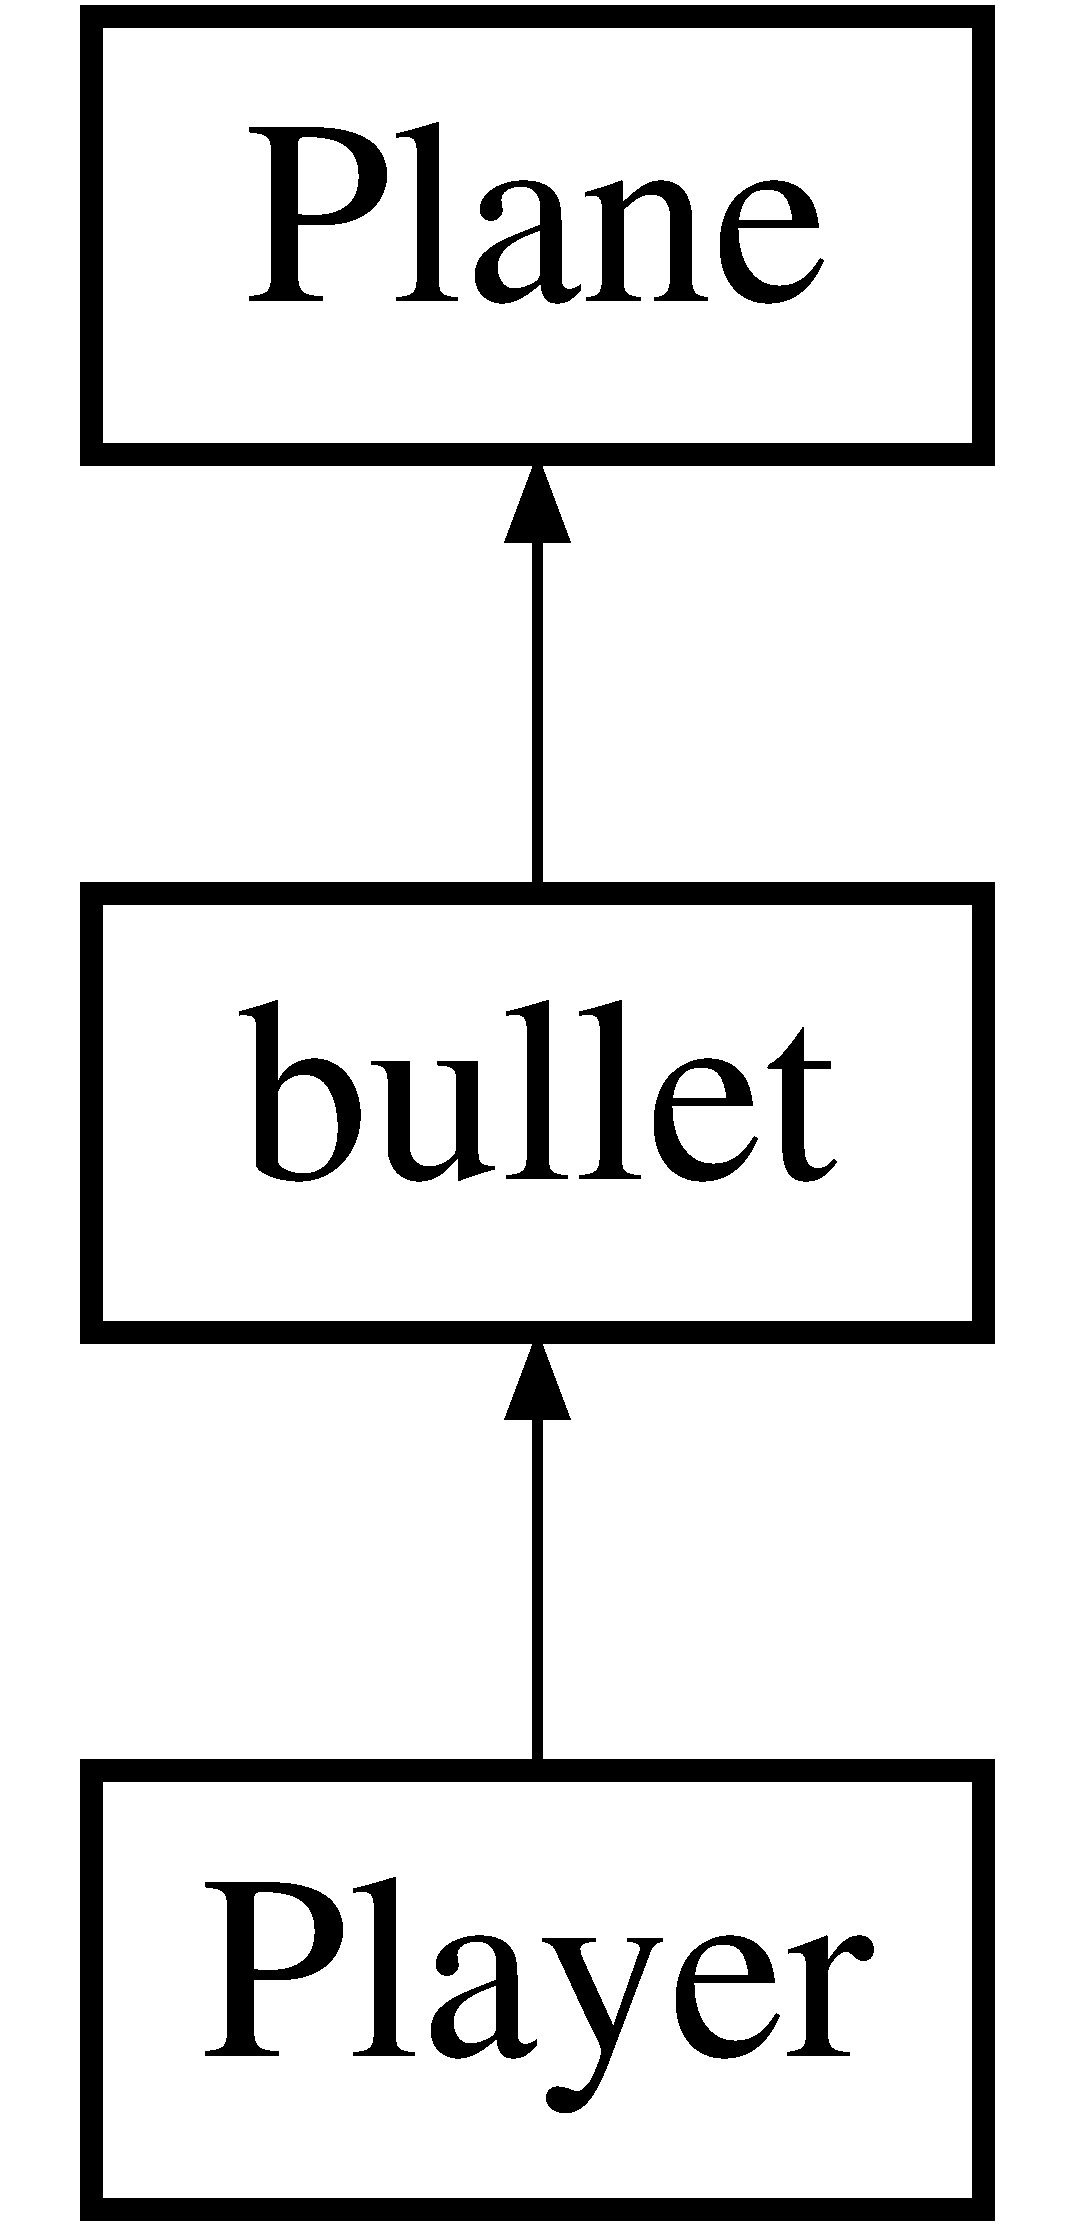
\includegraphics[height=3cm]{classbullet}
\end{center}
\end{figure}
\subsection*{Public Member Functions}
\begin{DoxyCompactItemize}
\item 
\hyperlink{classbullet_a56eac386b0e6268b746bd7ed4883e1df}{bullet} ()
\begin{DoxyCompactList}\small\item\em Constructor. \item\end{DoxyCompactList}\item 
\hyperlink{classbullet_a82a107fafc86d136e4a78ff13d14ceaf}{$\sim$bullet} ()
\begin{DoxyCompactList}\small\item\em Destructor. \item\end{DoxyCompactList}\item 
void \hyperlink{classbullet_a426140d3b62940f83861048560a570bd}{addBullet} (int, int)
\begin{DoxyCompactList}\small\item\em Creates the \hyperlink{classbullet}{bullet} and sets it at the x and y coordinates given with the two int parameters. \item\end{DoxyCompactList}\item 
void \hyperlink{classbullet_a32b293b38ec5efd19c86c5cc95ab0e25}{setBullet} (std::string fileName)
\begin{DoxyCompactList}\small\item\em Loads the bitmap image of the \hyperlink{classbullet}{bullet}. \item\end{DoxyCompactList}\item 
ALLEGRO\_\-BITMAP $\ast$ \hyperlink{classbullet_a16ea275b798ae9236015b3ff2e8fcb25}{getBulletMap} ()
\begin{DoxyCompactList}\small\item\em getter function to get the bitmat image of the \hyperlink{classbullet}{bullet} \item\end{DoxyCompactList}\item 
void \hyperlink{classbullet_a93cf5a76bb99163b52f5e42a359ea2e8}{drawB} ()
\begin{DoxyCompactList}\small\item\em Draw function that actually draws the \hyperlink{classbullet}{bullet} image. \item\end{DoxyCompactList}\end{DoxyCompactItemize}
\subsection*{Public Attributes}
\begin{DoxyCompactItemize}
\item 
list$<$ \hyperlink{classbulletType}{bulletType} $\ast$ $>$ \hyperlink{classbullet_ae700876dfc6875705a5c40ff4b80f94d}{Blist}
\end{DoxyCompactItemize}
\subsection*{Protected Attributes}
\begin{DoxyCompactItemize}
\item 
ALLEGRO\_\-BITMAP $\ast$ \hyperlink{classbullet_ae5e6772fcf149f67b495de01c350d83f}{Bbitmap}
\end{DoxyCompactItemize}


\subsection{Constructor \& Destructor Documentation}
\hypertarget{classbullet_a56eac386b0e6268b746bd7ed4883e1df}{
\index{bullet@{bullet}!bullet@{bullet}}
\index{bullet@{bullet}!bullet@{bullet}}
\subsubsection[{bullet}]{\setlength{\rightskip}{0pt plus 5cm}bullet::bullet ()}}
\label{classbullet_a56eac386b0e6268b746bd7ed4883e1df}


Constructor. 
\begin{DoxyParams}{Parameters}
\item[{\em No}]parameters \end{DoxyParams}
\begin{DoxyReturn}{Returns}
No return value 
\end{DoxyReturn}
\hypertarget{classbullet_a82a107fafc86d136e4a78ff13d14ceaf}{
\index{bullet@{bullet}!$\sim$bullet@{$\sim$bullet}}
\index{$\sim$bullet@{$\sim$bullet}!bullet@{bullet}}
\subsubsection[{$\sim$bullet}]{\setlength{\rightskip}{0pt plus 5cm}bullet::$\sim$bullet ()}}
\label{classbullet_a82a107fafc86d136e4a78ff13d14ceaf}


Destructor. 
\begin{DoxyParams}{Parameters}
\item[{\em No}]parameters \end{DoxyParams}
\begin{DoxyReturn}{Returns}
No return value 
\end{DoxyReturn}


\subsection{Member Function Documentation}
\hypertarget{classbullet_a426140d3b62940f83861048560a570bd}{
\index{bullet@{bullet}!addBullet@{addBullet}}
\index{addBullet@{addBullet}!bullet@{bullet}}
\subsubsection[{addBullet}]{\setlength{\rightskip}{0pt plus 5cm}void bullet::addBullet (int {\em e}, \/  int {\em f})}}
\label{classbullet_a426140d3b62940f83861048560a570bd}


Creates the \hyperlink{classbullet}{bullet} and sets it at the x and y coordinates given with the two int parameters. 
\begin{DoxyParams}{Parameters}
\item[{\em int}]: representing the x coordinate of the \hyperlink{classbullet}{bullet} \item[{\em int}]: representing the y coordinate of the \hyperlink{classbullet}{bullet} \end{DoxyParams}
\begin{DoxyReturn}{Returns}
No return value 
\end{DoxyReturn}
\hypertarget{classbullet_a93cf5a76bb99163b52f5e42a359ea2e8}{
\index{bullet@{bullet}!drawB@{drawB}}
\index{drawB@{drawB}!bullet@{bullet}}
\subsubsection[{drawB}]{\setlength{\rightskip}{0pt plus 5cm}bullet::drawB ()}}
\label{classbullet_a93cf5a76bb99163b52f5e42a359ea2e8}


Draw function that actually draws the \hyperlink{classbullet}{bullet} image. 
\begin{DoxyParams}{Parameters}
\item[{\em No}]parameters \end{DoxyParams}
\begin{DoxyReturn}{Returns}
No return value 
\end{DoxyReturn}
\hypertarget{classbullet_a16ea275b798ae9236015b3ff2e8fcb25}{
\index{bullet@{bullet}!getBulletMap@{getBulletMap}}
\index{getBulletMap@{getBulletMap}!bullet@{bullet}}
\subsubsection[{getBulletMap}]{\setlength{\rightskip}{0pt plus 5cm}ALLEGRO\_\-BITMAP $\ast$ bullet::getBulletMap ()}}
\label{classbullet_a16ea275b798ae9236015b3ff2e8fcb25}


getter function to get the bitmat image of the \hyperlink{classbullet}{bullet} 
\begin{DoxyParams}{Parameters}
\item[{\em No}]parameters \end{DoxyParams}
\begin{DoxyReturn}{Returns}
Bitmap image of the \hyperlink{classbullet}{bullet} 
\end{DoxyReturn}
\hypertarget{classbullet_a32b293b38ec5efd19c86c5cc95ab0e25}{
\index{bullet@{bullet}!setBullet@{setBullet}}
\index{setBullet@{setBullet}!bullet@{bullet}}
\subsubsection[{setBullet}]{\setlength{\rightskip}{0pt plus 5cm}bullet::setBullet (std::string {\em fileName})}}
\label{classbullet_a32b293b38ec5efd19c86c5cc95ab0e25}


Loads the bitmap image of the \hyperlink{classbullet}{bullet}. 
\begin{DoxyParams}{Parameters}
\item[{\em fileName}]: the file name/path that contains the image of the \hyperlink{classbullet}{bullet} \end{DoxyParams}
\begin{DoxyReturn}{Returns}
No return value 
\end{DoxyReturn}


\subsection{Member Data Documentation}
\hypertarget{classbullet_ae5e6772fcf149f67b495de01c350d83f}{
\index{bullet@{bullet}!Bbitmap@{Bbitmap}}
\index{Bbitmap@{Bbitmap}!bullet@{bullet}}
\subsubsection[{Bbitmap}]{\setlength{\rightskip}{0pt plus 5cm}ALLEGRO\_\-BITMAP$\ast$ {\bf bullet::Bbitmap}\hspace{0.3cm}{\ttfamily  \mbox{[}protected\mbox{]}}}}
\label{classbullet_ae5e6772fcf149f67b495de01c350d83f}
Creates a Bitmap object that will hold the \hyperlink{classbullet}{bullet} image \hypertarget{classbullet_ae700876dfc6875705a5c40ff4b80f94d}{
\index{bullet@{bullet}!Blist@{Blist}}
\index{Blist@{Blist}!bullet@{bullet}}
\subsubsection[{Blist}]{\setlength{\rightskip}{0pt plus 5cm}list$<${\bf bulletType}$\ast$$>$ {\bf bullet::Blist}}}
\label{classbullet_ae700876dfc6875705a5c40ff4b80f94d}
Creates a list of the bullets 

The documentation for this class was generated from the following files:\begin{DoxyCompactItemize}
\item 
\hyperlink{bullet_8h}{bullet.h}\item 
\hyperlink{bullet_8cc}{bullet.cc}\end{DoxyCompactItemize}

\hypertarget{classbulletType}{
\section{bulletType Class Reference}
\label{classbulletType}\index{bulletType@{bulletType}}
}


{\ttfamily \#include $<$bullet.h$>$}\subsection*{Public Member Functions}
\begin{DoxyCompactItemize}
\item 
\hyperlink{classbulletType_ad854048f38d7514caa09af4ab034837b}{bulletType} (int a, int b)
\begin{DoxyCompactList}\small\item\em Constructor. \item\end{DoxyCompactList}\item 
int \hyperlink{classbulletType_a3a40c67dcf6d3b6dc91e6fa7800cdaf4}{getbX} ()
\begin{DoxyCompactList}\small\item\em Gets the x coordinate of the \hyperlink{classbullet}{bullet}. \item\end{DoxyCompactList}\item 
void \hyperlink{classbulletType_a623f1eeb1381c512708efccafbb3c192}{setbY} (int a)
\begin{DoxyCompactList}\small\item\em Sets the Y coordinate of the \hyperlink{classbullet}{bullet} to the value of the int parameter. \item\end{DoxyCompactList}\item 
void \hyperlink{classbulletType_af69e22a00c81d5610cfb121dabf25b2b}{setbX} (int b)
\begin{DoxyCompactList}\small\item\em Sets the X coordinate of the \hyperlink{classbullet}{bullet} to the value of the int parameter. \item\end{DoxyCompactList}\item 
int \hyperlink{classbulletType_a6787ea4992f2fead3ee07e9216b06d4e}{getbY} ()
\begin{DoxyCompactList}\small\item\em Gets the y coordinate of the \hyperlink{classbullet}{bullet}. \item\end{DoxyCompactList}\end{DoxyCompactItemize}
\subsection*{Private Attributes}
\begin{DoxyCompactItemize}
\item 
int \hyperlink{classbulletType_a0078ec4eb7df2062788ae69200a73bf3}{bX}
\item 
int \hyperlink{classbulletType_a7083d68e84fe928b1e46575fda710d5d}{bY}
\end{DoxyCompactItemize}


\subsection{Constructor \& Destructor Documentation}
\hypertarget{classbulletType_ad854048f38d7514caa09af4ab034837b}{
\index{bulletType@{bulletType}!bulletType@{bulletType}}
\index{bulletType@{bulletType}!bulletType@{bulletType}}
\subsubsection[{bulletType}]{\setlength{\rightskip}{0pt plus 5cm}bulletType::bulletType (int {\em a}, \/  int {\em b})\hspace{0.3cm}{\ttfamily  \mbox{[}inline\mbox{]}}}}
\label{classbulletType_ad854048f38d7514caa09af4ab034837b}


Constructor. 
\begin{DoxyParams}{Parameters}
\item[{\em a}]X coordinate \item[{\em b}]Y coordinate \end{DoxyParams}
\begin{DoxyReturn}{Returns}
No return value 
\end{DoxyReturn}


\subsection{Member Function Documentation}
\hypertarget{classbulletType_a3a40c67dcf6d3b6dc91e6fa7800cdaf4}{
\index{bulletType@{bulletType}!getbX@{getbX}}
\index{getbX@{getbX}!bulletType@{bulletType}}
\subsubsection[{getbX}]{\setlength{\rightskip}{0pt plus 5cm}int bulletType::getbX ()\hspace{0.3cm}{\ttfamily  \mbox{[}inline\mbox{]}}}}
\label{classbulletType_a3a40c67dcf6d3b6dc91e6fa7800cdaf4}


Gets the x coordinate of the \hyperlink{classbullet}{bullet}. 
\begin{DoxyParams}{Parameters}
\item[{\em No}]parameters \end{DoxyParams}
\begin{DoxyReturn}{Returns}
Integer value 
\end{DoxyReturn}
\hypertarget{classbulletType_a6787ea4992f2fead3ee07e9216b06d4e}{
\index{bulletType@{bulletType}!getbY@{getbY}}
\index{getbY@{getbY}!bulletType@{bulletType}}
\subsubsection[{getbY}]{\setlength{\rightskip}{0pt plus 5cm}int bulletType::getbY ()\hspace{0.3cm}{\ttfamily  \mbox{[}inline\mbox{]}}}}
\label{classbulletType_a6787ea4992f2fead3ee07e9216b06d4e}


Gets the y coordinate of the \hyperlink{classbullet}{bullet}. 
\begin{DoxyParams}{Parameters}
\item[{\em No}]parameters \end{DoxyParams}
\begin{DoxyReturn}{Returns}
Integer value 
\end{DoxyReturn}
\hypertarget{classbulletType_af69e22a00c81d5610cfb121dabf25b2b}{
\index{bulletType@{bulletType}!setbX@{setbX}}
\index{setbX@{setbX}!bulletType@{bulletType}}
\subsubsection[{setbX}]{\setlength{\rightskip}{0pt plus 5cm}void bulletType::setbX (int {\em b})\hspace{0.3cm}{\ttfamily  \mbox{[}inline\mbox{]}}}}
\label{classbulletType_af69e22a00c81d5610cfb121dabf25b2b}


Sets the X coordinate of the \hyperlink{classbullet}{bullet} to the value of the int parameter. 
\begin{DoxyParams}{Parameters}
\item[{\em b}]: int value of the new X coordinate of the \hyperlink{classbullet}{bullet} \end{DoxyParams}
\begin{DoxyReturn}{Returns}
No return value 
\end{DoxyReturn}
\hypertarget{classbulletType_a623f1eeb1381c512708efccafbb3c192}{
\index{bulletType@{bulletType}!setbY@{setbY}}
\index{setbY@{setbY}!bulletType@{bulletType}}
\subsubsection[{setbY}]{\setlength{\rightskip}{0pt plus 5cm}void bulletType::setbY (int {\em a})\hspace{0.3cm}{\ttfamily  \mbox{[}inline\mbox{]}}}}
\label{classbulletType_a623f1eeb1381c512708efccafbb3c192}


Sets the Y coordinate of the \hyperlink{classbullet}{bullet} to the value of the int parameter. 
\begin{DoxyParams}{Parameters}
\item[{\em a}]: int value of the new Y coordinate of the \hyperlink{classbullet}{bullet} \end{DoxyParams}
\begin{DoxyReturn}{Returns}
No return value 
\end{DoxyReturn}


\subsection{Member Data Documentation}
\hypertarget{classbulletType_a0078ec4eb7df2062788ae69200a73bf3}{
\index{bulletType@{bulletType}!bX@{bX}}
\index{bX@{bX}!bulletType@{bulletType}}
\subsubsection[{bX}]{\setlength{\rightskip}{0pt plus 5cm}int {\bf bulletType::bX}\hspace{0.3cm}{\ttfamily  \mbox{[}private\mbox{]}}}}
\label{classbulletType_a0078ec4eb7df2062788ae69200a73bf3}
X coordinate of the \hyperlink{classbullet}{bullet} \hypertarget{classbulletType_a7083d68e84fe928b1e46575fda710d5d}{
\index{bulletType@{bulletType}!bY@{bY}}
\index{bY@{bY}!bulletType@{bulletType}}
\subsubsection[{bY}]{\setlength{\rightskip}{0pt plus 5cm}int {\bf bulletType::bY}\hspace{0.3cm}{\ttfamily  \mbox{[}private\mbox{]}}}}
\label{classbulletType_a7083d68e84fe928b1e46575fda710d5d}
Y coordinate of the \hyperlink{classbullet}{bullet} 

The documentation for this class was generated from the following file:\begin{DoxyCompactItemize}
\item 
\hyperlink{bullet_8h}{bullet.h}\end{DoxyCompactItemize}

\hypertarget{classEnemy}{
\section{Enemy Class Reference}
\label{classEnemy}\index{Enemy@{Enemy}}
}


{\ttfamily \#include $<$Enemy.h$>$}Inheritance diagram for Enemy::\begin{figure}[H]
\begin{center}
\leavevmode
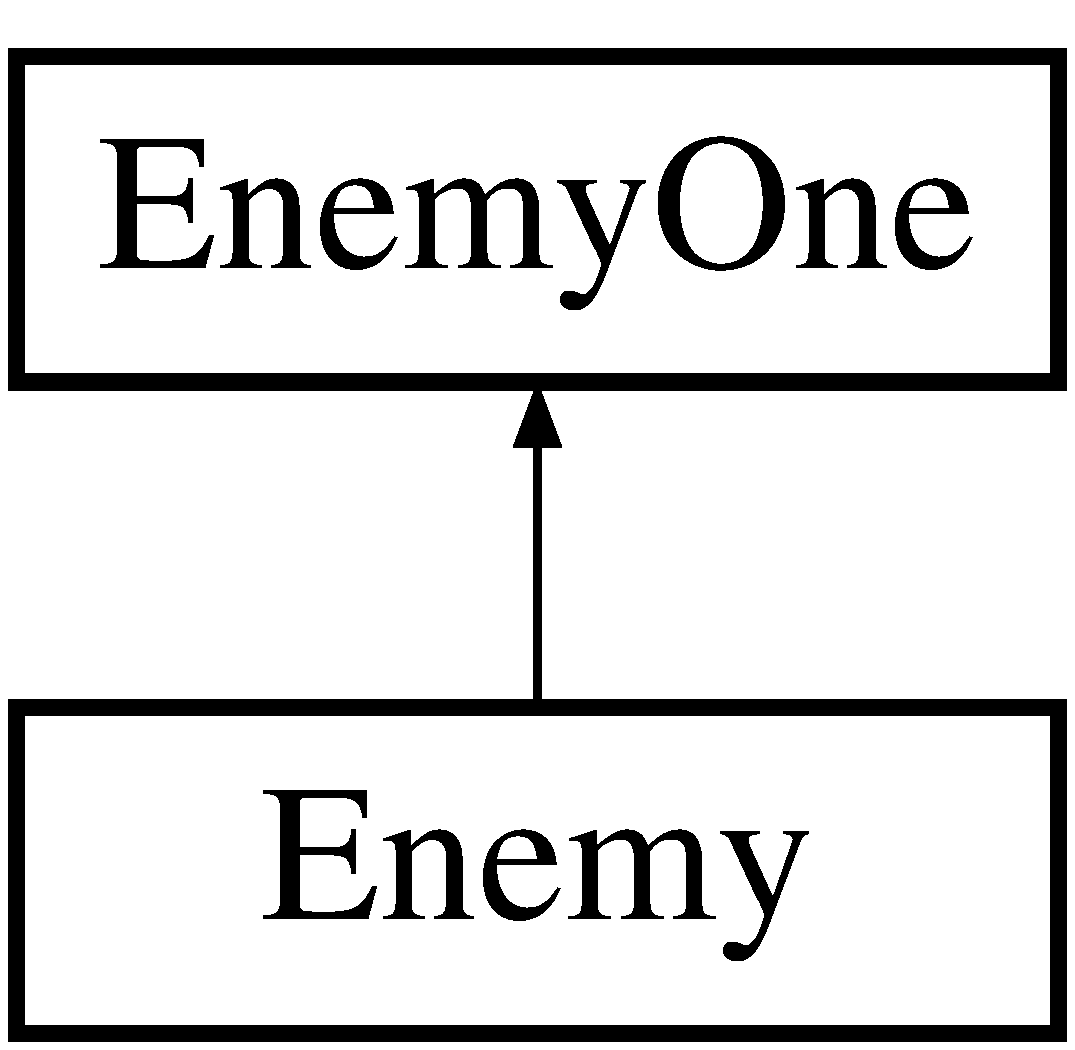
\includegraphics[height=2cm]{classEnemy}
\end{center}
\end{figure}
\subsection*{Public Member Functions}
\begin{DoxyCompactItemize}
\item 
\hyperlink{classEnemy_a94f30d348b6d2840fd71675472ba38dd}{Enemy} ()
\begin{DoxyCompactList}\small\item\em Constructor. \item\end{DoxyCompactList}\item 
\hyperlink{classEnemy_ac0eec4755e28c02688065f9657150ac3}{$\sim$Enemy} ()
\begin{DoxyCompactList}\small\item\em Destructor. \item\end{DoxyCompactList}\item 
void \hyperlink{classEnemy_a0dcca8a418323526c286c323a3fb2fd1}{moveEnemy} ()
\begin{DoxyCompactList}\small\item\em Defines the movement of the first enemy type to move from right to left by subtracting the 'moveSpeed' from the x coordinate. if enemy goes out of the screen on the left, it is reset to the right side. \item\end{DoxyCompactList}\item 
void \hyperlink{classEnemy_a405168f47abea55981313377385d6c37}{moveboss} ()
\begin{DoxyCompactList}\small\item\em Defines the movement of the second enemy type to move from right to left by subracting the 'moveSpeed' from the x coordinate. \item\end{DoxyCompactList}\end{DoxyCompactItemize}
\subsection*{Protected Attributes}
\begin{DoxyCompactItemize}
\item 
int \hyperlink{classEnemy_aedd5e7bf8ef07ee97be433c853a10d8d}{health}
\end{DoxyCompactItemize}


\subsection{Constructor \& Destructor Documentation}
\hypertarget{classEnemy_a94f30d348b6d2840fd71675472ba38dd}{
\index{Enemy@{Enemy}!Enemy@{Enemy}}
\index{Enemy@{Enemy}!Enemy@{Enemy}}
\subsubsection[{Enemy}]{\setlength{\rightskip}{0pt plus 5cm}Enemy::Enemy ()}}
\label{classEnemy_a94f30d348b6d2840fd71675472ba38dd}


Constructor. 
\begin{DoxyParams}{Parameters}
\item[{\em No}]parameters \end{DoxyParams}
\begin{DoxyReturn}{Returns}
No return value 
\end{DoxyReturn}
\hypertarget{classEnemy_ac0eec4755e28c02688065f9657150ac3}{
\index{Enemy@{Enemy}!$\sim$Enemy@{$\sim$Enemy}}
\index{$\sim$Enemy@{$\sim$Enemy}!Enemy@{Enemy}}
\subsubsection[{$\sim$Enemy}]{\setlength{\rightskip}{0pt plus 5cm}Enemy::$\sim$Enemy ()}}
\label{classEnemy_ac0eec4755e28c02688065f9657150ac3}


Destructor. 
\begin{DoxyParams}{Parameters}
\item[{\em No}]parameters \end{DoxyParams}
\begin{DoxyReturn}{Returns}
No return value 
\end{DoxyReturn}


\subsection{Member Function Documentation}
\hypertarget{classEnemy_a405168f47abea55981313377385d6c37}{
\index{Enemy@{Enemy}!moveboss@{moveboss}}
\index{moveboss@{moveboss}!Enemy@{Enemy}}
\subsubsection[{moveboss}]{\setlength{\rightskip}{0pt plus 5cm}void Enemy::moveboss ()}}
\label{classEnemy_a405168f47abea55981313377385d6c37}


Defines the movement of the second enemy type to move from right to left by subracting the 'moveSpeed' from the x coordinate. 
\begin{DoxyParams}{Parameters}
\item[{\em No}]parameters \end{DoxyParams}
\begin{DoxyReturn}{Returns}
No return value 
\end{DoxyReturn}
\hypertarget{classEnemy_a0dcca8a418323526c286c323a3fb2fd1}{
\index{Enemy@{Enemy}!moveEnemy@{moveEnemy}}
\index{moveEnemy@{moveEnemy}!Enemy@{Enemy}}
\subsubsection[{moveEnemy}]{\setlength{\rightskip}{0pt plus 5cm}void Enemy::moveEnemy ()}}
\label{classEnemy_a0dcca8a418323526c286c323a3fb2fd1}


Defines the movement of the first enemy type to move from right to left by subtracting the 'moveSpeed' from the x coordinate. if enemy goes out of the screen on the left, it is reset to the right side. 
\begin{DoxyParams}{Parameters}
\item[{\em No}]parameters \end{DoxyParams}
\begin{DoxyReturn}{Returns}
No return value 
\end{DoxyReturn}


\subsection{Member Data Documentation}
\hypertarget{classEnemy_aedd5e7bf8ef07ee97be433c853a10d8d}{
\index{Enemy@{Enemy}!health@{health}}
\index{health@{health}!Enemy@{Enemy}}
\subsubsection[{health}]{\setlength{\rightskip}{0pt plus 5cm}int {\bf Enemy::health}\hspace{0.3cm}{\ttfamily  \mbox{[}protected\mbox{]}}}}
\label{classEnemy_aedd5e7bf8ef07ee97be433c853a10d8d}
the health of the enemy which is set to 0 by the constructor 

The documentation for this class was generated from the following files:\begin{DoxyCompactItemize}
\item 
\hyperlink{Enemy_8h}{Enemy.h}\item 
\hyperlink{Enemy_8cc}{Enemy.cc}\end{DoxyCompactItemize}

\hypertarget{classEnemyOne}{
\section{EnemyOne Class Reference}
\label{classEnemyOne}\index{EnemyOne@{EnemyOne}}
}


{\ttfamily \#include $<$EnemyOne.h$>$}Inheritance diagram for EnemyOne::\begin{figure}[H]
\begin{center}
\leavevmode
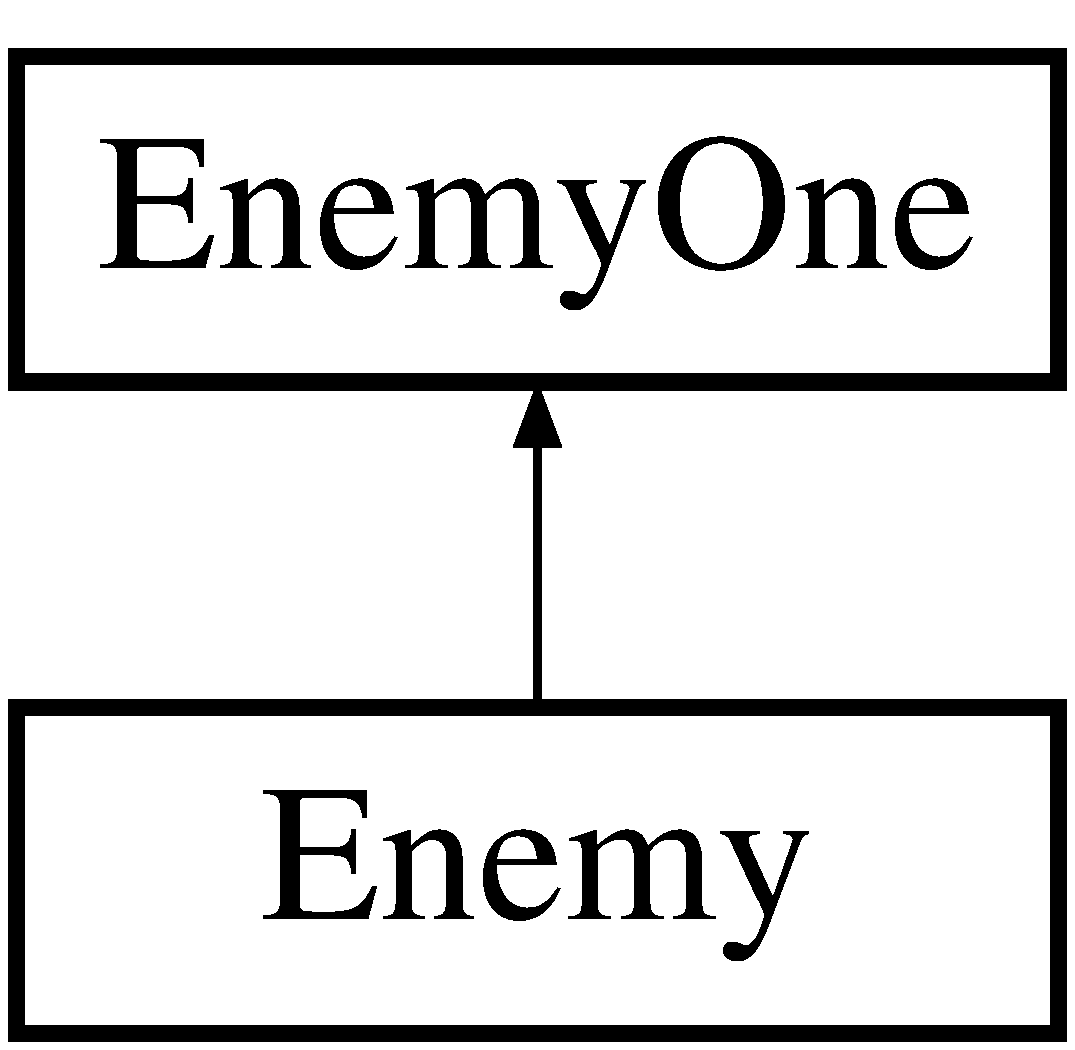
\includegraphics[height=2cm]{classEnemyOne}
\end{center}
\end{figure}
\subsection*{Public Member Functions}
\begin{DoxyCompactItemize}
\item 
\hyperlink{classEnemyOne_a876b7dc33899c1627a0ee1e08b34baf8}{EnemyOne} ()
\begin{DoxyCompactList}\small\item\em Constructor : Sets the images for the two enemy types to NULL before they are actually initialized. \item\end{DoxyCompactList}\item 
virtual \hyperlink{classEnemyOne_ad7999ae2c8228030d3f07df562a5aa0a}{$\sim$EnemyOne} ()
\begin{DoxyCompactList}\small\item\em Destructor : Destroys any enemy type created dynamically. \item\end{DoxyCompactList}\item 
void \hyperlink{classEnemyOne_a428e216932e0a454b59b705f62d1c1a0}{addEnemy} (int, int)
\begin{DoxyCompactList}\small\item\em Creates an \hyperlink{classEnemy}{Enemy} object dynamically at the coordinates given by b \& s which represent the x and y coordinates respectively. \item\end{DoxyCompactList}\item 
void \hyperlink{classEnemyOne_a53c380bf26465df0f0f7beaca93b952d}{setEnemy} (std::string name)
\begin{DoxyCompactList}\small\item\em Loads the image name in the parameter list onto the Ebitmap object. \item\end{DoxyCompactList}\item 
ALLEGRO\_\-BITMAP $\ast$ \hyperlink{classEnemyOne_a348b86c31e258c7ccf83a4f44397f542}{getEnemy} ()
\begin{DoxyCompactList}\small\item\em Getter function to get the set \hyperlink{classEnemy}{Enemy} image. \item\end{DoxyCompactList}\item 
void \hyperlink{classEnemyOne_a8017eb7f3cf8510043e542ed5314fbf9}{drawE} ()
\begin{DoxyCompactList}\small\item\em A draw function that draws the image loaded onto the enemy bitmap. \item\end{DoxyCompactList}\end{DoxyCompactItemize}
\subsection*{Public Attributes}
\begin{DoxyCompactItemize}
\item 
list$<$ \hyperlink{classEnemytype}{Enemytype} $\ast$ $>$ \hyperlink{classEnemyOne_a1e46e43f2fe68dad65a79d57671159b6}{Elist}
\end{DoxyCompactItemize}
\subsection*{Protected Attributes}
\begin{DoxyCompactItemize}
\item 
ALLEGRO\_\-BITMAP $\ast$ \hyperlink{classEnemyOne_a186a44174a5f8c35d805209c1806d967}{Ebitmap}
\item 
ALLEGRO\_\-BITMAP $\ast$ \hyperlink{classEnemyOne_ab42c5298a1849dd5a422dfaa1dc0f459}{Ebitmap2}
\end{DoxyCompactItemize}


\subsection{Constructor \& Destructor Documentation}
\hypertarget{classEnemyOne_a876b7dc33899c1627a0ee1e08b34baf8}{
\index{EnemyOne@{EnemyOne}!EnemyOne@{EnemyOne}}
\index{EnemyOne@{EnemyOne}!EnemyOne@{EnemyOne}}
\subsubsection[{EnemyOne}]{\setlength{\rightskip}{0pt plus 5cm}EnemyOne::EnemyOne ()}}
\label{classEnemyOne_a876b7dc33899c1627a0ee1e08b34baf8}


Constructor : Sets the images for the two enemy types to NULL before they are actually initialized. 
\begin{DoxyParams}{Parameters}
\item[{\em No}]parameters \end{DoxyParams}
\begin{DoxyReturn}{Returns}
No return value 
\end{DoxyReturn}
\hypertarget{classEnemyOne_ad7999ae2c8228030d3f07df562a5aa0a}{
\index{EnemyOne@{EnemyOne}!$\sim$EnemyOne@{$\sim$EnemyOne}}
\index{$\sim$EnemyOne@{$\sim$EnemyOne}!EnemyOne@{EnemyOne}}
\subsubsection[{$\sim$EnemyOne}]{\setlength{\rightskip}{0pt plus 5cm}EnemyOne::$\sim$EnemyOne ()\hspace{0.3cm}{\ttfamily  \mbox{[}virtual\mbox{]}}}}
\label{classEnemyOne_ad7999ae2c8228030d3f07df562a5aa0a}


Destructor : Destroys any enemy type created dynamically. 
\begin{DoxyParams}{Parameters}
\item[{\em No}]parameters \end{DoxyParams}
\begin{DoxyReturn}{Returns}
No return value 
\end{DoxyReturn}


\subsection{Member Function Documentation}
\hypertarget{classEnemyOne_a428e216932e0a454b59b705f62d1c1a0}{
\index{EnemyOne@{EnemyOne}!addEnemy@{addEnemy}}
\index{addEnemy@{addEnemy}!EnemyOne@{EnemyOne}}
\subsubsection[{addEnemy}]{\setlength{\rightskip}{0pt plus 5cm}void EnemyOne::addEnemy (int {\em b}, \/  int {\em s})}}
\label{classEnemyOne_a428e216932e0a454b59b705f62d1c1a0}


Creates an \hyperlink{classEnemy}{Enemy} object dynamically at the coordinates given by b \& s which represent the x and y coordinates respectively. 
\begin{DoxyParams}{Parameters}
\item[{\em b}]: x coordinate \item[{\em s}]: y coordinate \end{DoxyParams}
\begin{DoxyReturn}{Returns}
No return value 
\end{DoxyReturn}
\hypertarget{classEnemyOne_a8017eb7f3cf8510043e542ed5314fbf9}{
\index{EnemyOne@{EnemyOne}!drawE@{drawE}}
\index{drawE@{drawE}!EnemyOne@{EnemyOne}}
\subsubsection[{drawE}]{\setlength{\rightskip}{0pt plus 5cm}void EnemyOne::drawE ()}}
\label{classEnemyOne_a8017eb7f3cf8510043e542ed5314fbf9}


A draw function that draws the image loaded onto the enemy bitmap. 
\begin{DoxyParams}{Parameters}
\item[{\em No}]parameters \end{DoxyParams}
\begin{DoxyReturn}{Returns}
No return value 
\end{DoxyReturn}
\hypertarget{classEnemyOne_a348b86c31e258c7ccf83a4f44397f542}{
\index{EnemyOne@{EnemyOne}!getEnemy@{getEnemy}}
\index{getEnemy@{getEnemy}!EnemyOne@{EnemyOne}}
\subsubsection[{getEnemy}]{\setlength{\rightskip}{0pt plus 5cm}ALLEGRO\_\-BITMAP $\ast$ EnemyOne::getEnemy ()}}
\label{classEnemyOne_a348b86c31e258c7ccf83a4f44397f542}


Getter function to get the set \hyperlink{classEnemy}{Enemy} image. 
\begin{DoxyParams}{Parameters}
\item[{\em No}]parameters \end{DoxyParams}
\begin{DoxyReturn}{Returns}
ALLEGRO\_\-BITMAP type : the enemy image 
\end{DoxyReturn}
\hypertarget{classEnemyOne_a53c380bf26465df0f0f7beaca93b952d}{
\index{EnemyOne@{EnemyOne}!setEnemy@{setEnemy}}
\index{setEnemy@{setEnemy}!EnemyOne@{EnemyOne}}
\subsubsection[{setEnemy}]{\setlength{\rightskip}{0pt plus 5cm}void EnemyOne::setEnemy (std::string {\em name})}}
\label{classEnemyOne_a53c380bf26465df0f0f7beaca93b952d}


Loads the image name in the parameter list onto the Ebitmap object. 
\begin{DoxyParams}{Parameters}
\item[{\em name}]: the name of the image as stored in the folder \end{DoxyParams}
\begin{DoxyReturn}{Returns}
No return value 
\end{DoxyReturn}


\subsection{Member Data Documentation}
\hypertarget{classEnemyOne_a186a44174a5f8c35d805209c1806d967}{
\index{EnemyOne@{EnemyOne}!Ebitmap@{Ebitmap}}
\index{Ebitmap@{Ebitmap}!EnemyOne@{EnemyOne}}
\subsubsection[{Ebitmap}]{\setlength{\rightskip}{0pt plus 5cm}ALLEGRO\_\-BITMAP$\ast$ {\bf EnemyOne::Ebitmap}\hspace{0.3cm}{\ttfamily  \mbox{[}protected\mbox{]}}}}
\label{classEnemyOne_a186a44174a5f8c35d805209c1806d967}
The first enemy type \hypertarget{classEnemyOne_ab42c5298a1849dd5a422dfaa1dc0f459}{
\index{EnemyOne@{EnemyOne}!Ebitmap2@{Ebitmap2}}
\index{Ebitmap2@{Ebitmap2}!EnemyOne@{EnemyOne}}
\subsubsection[{Ebitmap2}]{\setlength{\rightskip}{0pt plus 5cm}ALLEGRO\_\-BITMAP$\ast$ {\bf EnemyOne::Ebitmap2}\hspace{0.3cm}{\ttfamily  \mbox{[}protected\mbox{]}}}}
\label{classEnemyOne_ab42c5298a1849dd5a422dfaa1dc0f459}
The second enemy type \hypertarget{classEnemyOne_a1e46e43f2fe68dad65a79d57671159b6}{
\index{EnemyOne@{EnemyOne}!Elist@{Elist}}
\index{Elist@{Elist}!EnemyOne@{EnemyOne}}
\subsubsection[{Elist}]{\setlength{\rightskip}{0pt plus 5cm}list$<${\bf Enemytype}$\ast$$>$ {\bf EnemyOne::Elist}}}
\label{classEnemyOne_a1e46e43f2fe68dad65a79d57671159b6}
A list that allows for the creation of multiple enemies dynamically 

The documentation for this class was generated from the following files:\begin{DoxyCompactItemize}
\item 
\hyperlink{EnemyOne_8h}{EnemyOne.h}\item 
\hyperlink{EnemyOne_8cc}{EnemyOne.cc}\end{DoxyCompactItemize}

\hypertarget{classEnemytype}{
\section{Enemytype Class Reference}
\label{classEnemytype}\index{Enemytype@{Enemytype}}
}


{\ttfamily \#include $<$EnemyOne.h$>$}\subsection*{Public Member Functions}
\begin{DoxyCompactItemize}
\item 
int \hyperlink{classEnemytype_a641488fb71b330a7104abe92acd0601a}{getX} ()
\begin{DoxyCompactList}\small\item\em Getter function for the X coordinate of the enemy. \item\end{DoxyCompactList}\item 
int \hyperlink{classEnemytype_aca1ceba65fea5f547abcfaa957c7e5ce}{getY} ()
\begin{DoxyCompactList}\small\item\em Getter function for the Y coordinate of the enemy. \item\end{DoxyCompactList}\item 
void \hyperlink{classEnemytype_a19472039711c84c97ef8d11921b9e510}{setX} (int a)
\begin{DoxyCompactList}\small\item\em Setter function which sets the x coordinate of the enemy. \item\end{DoxyCompactList}\item 
void \hyperlink{classEnemytype_a873a843e7f6eba7dd8ef41d4041661f6}{setY} (int b)
\begin{DoxyCompactList}\small\item\em Setter function which sets the Y coordinate of the enemy. \item\end{DoxyCompactList}\item 
int \hyperlink{classEnemytype_adc3cce767c80a8dee47acd0e48691ac3}{getMS} ()
\begin{DoxyCompactList}\small\item\em a getter function which gets the set speed of the enemy \item\end{DoxyCompactList}\item 
\hyperlink{classEnemytype_a315e220bfb4ffe6c67f31ac57b015679}{Enemytype} (int a, int s)
\begin{DoxyCompactList}\small\item\em Constructor : Creates the enemy to come from the right side of the screen(the x coordinate is automatically set to 640) and sets the speed at which they move. \item\end{DoxyCompactList}\end{DoxyCompactItemize}
\subsection*{Private Attributes}
\begin{DoxyCompactItemize}
\item 
int \hyperlink{classEnemytype_ac73360c104ab8e6f4cad79af69e904dd}{x}
\item 
int \hyperlink{classEnemytype_a22ab8ba090798eb7fad364b0319f4d13}{y}
\item 
int \hyperlink{classEnemytype_a7fbb15c1e006c25cc926b55cd3ea23dd}{moveSpeed}
\end{DoxyCompactItemize}


\subsection{Constructor \& Destructor Documentation}
\hypertarget{classEnemytype_a315e220bfb4ffe6c67f31ac57b015679}{
\index{Enemytype@{Enemytype}!Enemytype@{Enemytype}}
\index{Enemytype@{Enemytype}!Enemytype@{Enemytype}}
\subsubsection[{Enemytype}]{\setlength{\rightskip}{0pt plus 5cm}Enemytype::Enemytype (int {\em a}, \/  int {\em s})\hspace{0.3cm}{\ttfamily  \mbox{[}inline\mbox{]}}}}
\label{classEnemytype_a315e220bfb4ffe6c67f31ac57b015679}


Constructor : Creates the enemy to come from the right side of the screen(the x coordinate is automatically set to 640) and sets the speed at which they move. 
\begin{DoxyParams}{Parameters}
\item[{\em a,:}]the y coordinate of the enemy \item[{\em s,:}]the speed at which the enemies move \end{DoxyParams}
\begin{DoxyReturn}{Returns}
No return value 
\end{DoxyReturn}


\subsection{Member Function Documentation}
\hypertarget{classEnemytype_adc3cce767c80a8dee47acd0e48691ac3}{
\index{Enemytype@{Enemytype}!getMS@{getMS}}
\index{getMS@{getMS}!Enemytype@{Enemytype}}
\subsubsection[{getMS}]{\setlength{\rightskip}{0pt plus 5cm}int Enemytype::getMS ()\hspace{0.3cm}{\ttfamily  \mbox{[}inline\mbox{]}}}}
\label{classEnemytype_adc3cce767c80a8dee47acd0e48691ac3}


a getter function which gets the set speed of the enemy 
\begin{DoxyParams}{Parameters}
\item[{\em No}]parameters \end{DoxyParams}
\begin{DoxyReturn}{Returns}
moveSpeed : the speed of the enemy 
\end{DoxyReturn}
\hypertarget{classEnemytype_a641488fb71b330a7104abe92acd0601a}{
\index{Enemytype@{Enemytype}!getX@{getX}}
\index{getX@{getX}!Enemytype@{Enemytype}}
\subsubsection[{getX}]{\setlength{\rightskip}{0pt plus 5cm}int Enemytype::getX ()\hspace{0.3cm}{\ttfamily  \mbox{[}inline\mbox{]}}}}
\label{classEnemytype_a641488fb71b330a7104abe92acd0601a}


Getter function for the X coordinate of the enemy. 
\begin{DoxyParams}{Parameters}
\item[{\em No}]parameters \end{DoxyParams}
\begin{DoxyReturn}{Returns}
No return value 
\end{DoxyReturn}
\hypertarget{classEnemytype_aca1ceba65fea5f547abcfaa957c7e5ce}{
\index{Enemytype@{Enemytype}!getY@{getY}}
\index{getY@{getY}!Enemytype@{Enemytype}}
\subsubsection[{getY}]{\setlength{\rightskip}{0pt plus 5cm}int Enemytype::getY ()\hspace{0.3cm}{\ttfamily  \mbox{[}inline\mbox{]}}}}
\label{classEnemytype_aca1ceba65fea5f547abcfaa957c7e5ce}


Getter function for the Y coordinate of the enemy. 
\begin{DoxyParams}{Parameters}
\item[{\em No}]parameters \end{DoxyParams}
\begin{DoxyReturn}{Returns}
int : the y coordinate of the enemy 
\end{DoxyReturn}
\hypertarget{classEnemytype_a19472039711c84c97ef8d11921b9e510}{
\index{Enemytype@{Enemytype}!setX@{setX}}
\index{setX@{setX}!Enemytype@{Enemytype}}
\subsubsection[{setX}]{\setlength{\rightskip}{0pt plus 5cm}void Enemytype::setX (int {\em a})\hspace{0.3cm}{\ttfamily  \mbox{[}inline\mbox{]}}}}
\label{classEnemytype_a19472039711c84c97ef8d11921b9e510}


Setter function which sets the x coordinate of the enemy. 
\begin{DoxyParams}{Parameters}
\item[{\em a}]: the value which the X coordinate of the enemy will be set to \end{DoxyParams}
\begin{DoxyReturn}{Returns}
No return value 
\end{DoxyReturn}
\hypertarget{classEnemytype_a873a843e7f6eba7dd8ef41d4041661f6}{
\index{Enemytype@{Enemytype}!setY@{setY}}
\index{setY@{setY}!Enemytype@{Enemytype}}
\subsubsection[{setY}]{\setlength{\rightskip}{0pt plus 5cm}void Enemytype::setY (int {\em b})\hspace{0.3cm}{\ttfamily  \mbox{[}inline\mbox{]}}}}
\label{classEnemytype_a873a843e7f6eba7dd8ef41d4041661f6}


Setter function which sets the Y coordinate of the enemy. 
\begin{DoxyParams}{Parameters}
\item[{\em b}]: the value which the Y coordinate of the enemy will be set to \end{DoxyParams}
\begin{DoxyReturn}{Returns}
No return value 
\end{DoxyReturn}


\subsection{Member Data Documentation}
\hypertarget{classEnemytype_a7fbb15c1e006c25cc926b55cd3ea23dd}{
\index{Enemytype@{Enemytype}!moveSpeed@{moveSpeed}}
\index{moveSpeed@{moveSpeed}!Enemytype@{Enemytype}}
\subsubsection[{moveSpeed}]{\setlength{\rightskip}{0pt plus 5cm}int {\bf Enemytype::moveSpeed}\hspace{0.3cm}{\ttfamily  \mbox{[}private\mbox{]}}}}
\label{classEnemytype_a7fbb15c1e006c25cc926b55cd3ea23dd}
the speed at which the enemy object is moving \hypertarget{classEnemytype_ac73360c104ab8e6f4cad79af69e904dd}{
\index{Enemytype@{Enemytype}!x@{x}}
\index{x@{x}!Enemytype@{Enemytype}}
\subsubsection[{x}]{\setlength{\rightskip}{0pt plus 5cm}int {\bf Enemytype::x}\hspace{0.3cm}{\ttfamily  \mbox{[}private\mbox{]}}}}
\label{classEnemytype_ac73360c104ab8e6f4cad79af69e904dd}
the x coordinate of the enemy object \hypertarget{classEnemytype_a22ab8ba090798eb7fad364b0319f4d13}{
\index{Enemytype@{Enemytype}!y@{y}}
\index{y@{y}!Enemytype@{Enemytype}}
\subsubsection[{y}]{\setlength{\rightskip}{0pt plus 5cm}int {\bf Enemytype::y}\hspace{0.3cm}{\ttfamily  \mbox{[}private\mbox{]}}}}
\label{classEnemytype_a22ab8ba090798eb7fad364b0319f4d13}
the y coordinate of the enemy object 

The documentation for this class was generated from the following file:\begin{DoxyCompactItemize}
\item 
\hyperlink{EnemyOne_8h}{EnemyOne.h}\end{DoxyCompactItemize}

\hypertarget{classKeyboard}{
\section{Keyboard Class Reference}
\label{classKeyboard}\index{Keyboard@{Keyboard}}
}


{\ttfamily \#include $<$Keyboard.h$>$}\subsection*{Public Member Functions}
\begin{DoxyCompactItemize}
\item 
\hyperlink{classKeyboard_ad6b0bb849d6bb7cdf63091e40b5f5f7f}{Keyboard} ()
\item 
\hyperlink{classKeyboard_af6a99ec66c8c722a45b967bf79167038}{$\sim$Keyboard} ()
\end{DoxyCompactItemize}
\subsection*{Public Attributes}
\begin{DoxyCompactItemize}
\item 
bool \hyperlink{classKeyboard_aad6d0d22cffc14a293b3a3b6a98da05d}{key} \mbox{[}6\mbox{]}
\end{DoxyCompactItemize}


\subsection{Constructor \& Destructor Documentation}
\hypertarget{classKeyboard_ad6b0bb849d6bb7cdf63091e40b5f5f7f}{
\index{Keyboard@{Keyboard}!Keyboard@{Keyboard}}
\index{Keyboard@{Keyboard}!Keyboard@{Keyboard}}
\subsubsection[{Keyboard}]{\setlength{\rightskip}{0pt plus 5cm}Keyboard::Keyboard ()}}
\label{classKeyboard_ad6b0bb849d6bb7cdf63091e40b5f5f7f}
\hypertarget{classKeyboard_af6a99ec66c8c722a45b967bf79167038}{
\index{Keyboard@{Keyboard}!$\sim$Keyboard@{$\sim$Keyboard}}
\index{$\sim$Keyboard@{$\sim$Keyboard}!Keyboard@{Keyboard}}
\subsubsection[{$\sim$Keyboard}]{\setlength{\rightskip}{0pt plus 5cm}Keyboard::$\sim$Keyboard ()}}
\label{classKeyboard_af6a99ec66c8c722a45b967bf79167038}


\subsection{Member Data Documentation}
\hypertarget{classKeyboard_aad6d0d22cffc14a293b3a3b6a98da05d}{
\index{Keyboard@{Keyboard}!key@{key}}
\index{key@{key}!Keyboard@{Keyboard}}
\subsubsection[{key}]{\setlength{\rightskip}{0pt plus 5cm}bool {\bf Keyboard::key}\mbox{[}6\mbox{]}}}
\label{classKeyboard_aad6d0d22cffc14a293b3a3b6a98da05d}


The documentation for this class was generated from the following files:\begin{DoxyCompactItemize}
\item 
\hyperlink{Keyboard_8h}{Keyboard.h}\item 
\hyperlink{Keyboard_8cc}{Keyboard.cc}\end{DoxyCompactItemize}

\hypertarget{classPlane}{
\section{Plane Class Reference}
\label{classPlane}\index{Plane@{Plane}}
}


{\ttfamily \#include $<$Plane.h$>$}Inheritance diagram for Plane::\begin{figure}[H]
\begin{center}
\leavevmode
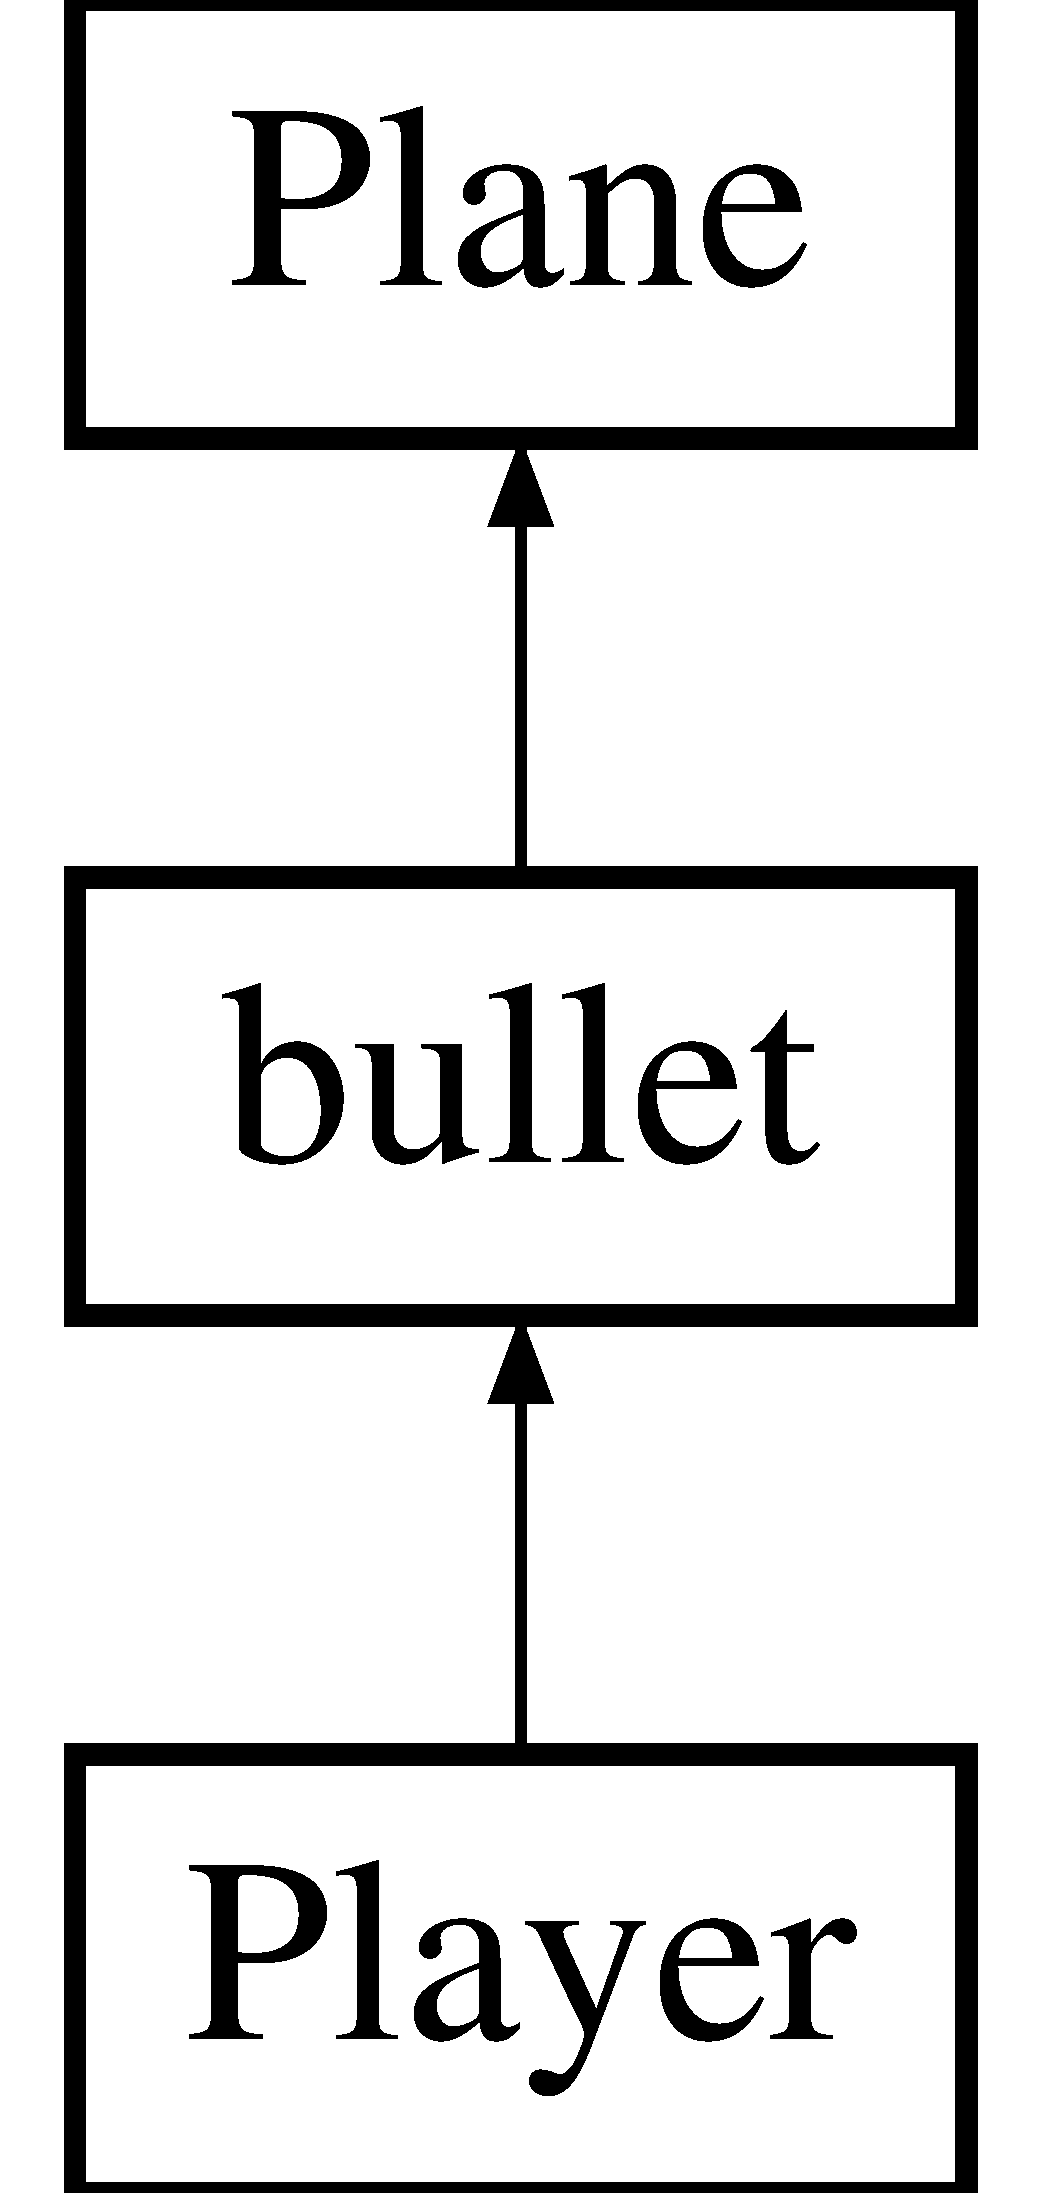
\includegraphics[height=3cm]{classPlane}
\end{center}
\end{figure}
\subsection*{Public Member Functions}
\begin{DoxyCompactItemize}
\item 
\hyperlink{classPlane_acac0d9c003e0ab10d07b146c3566a0c7}{Plane} ()
\begin{DoxyCompactList}\small\item\em Constructor. \item\end{DoxyCompactList}\item 
virtual \hyperlink{classPlane_a69abd86051c880dcb44b249ad10c4436}{$\sim$Plane} ()
\begin{DoxyCompactList}\small\item\em Destructor. \item\end{DoxyCompactList}\item 
int \hyperlink{classPlane_ab0db534796dff1c2ff490fe989261cda}{getX} ()
\begin{DoxyCompactList}\small\item\em this function gets the X coordinate of the object \item\end{DoxyCompactList}\item 
int \hyperlink{classPlane_a8c754851771ba75ecd163a55d2f31800}{getY} ()
\begin{DoxyCompactList}\small\item\em this function gets the Y coordinate of the object \item\end{DoxyCompactList}\item 
void \hyperlink{classPlane_a41fc70cf581d5f3d5efaba227d0b406b}{setBitmap} (std::string filePath)
\item 
ALLEGRO\_\-BITMAP $\ast$ \hyperlink{classPlane_a0d2bb766e1d07c7097fd741adff8c4d8}{getBitmap} ()
\begin{DoxyCompactList}\small\item\em This function is used to get the object loaded onto the bitmap object by the function 'setBitmap'. \item\end{DoxyCompactList}\item 
void \hyperlink{classPlane_a6f961e4c2c03b03bac2bd61749ec51e1}{initialPlane} ()
\begin{DoxyCompactList}\small\item\em This function set the starting point of the player by setting both the x and y coordinates to 10 and 240 respectively. \item\end{DoxyCompactList}\item 
void \hyperlink{classPlane_a8877358878e91929c4c01bad40cbdb78}{draw} ()
\begin{DoxyCompactList}\small\item\em this function draws the loaded bitmap to the screen on the point provided by the x and y coordinates provided \item\end{DoxyCompactList}\end{DoxyCompactItemize}
\subsection*{Protected Attributes}
\begin{DoxyCompactItemize}
\item 
ALLEGRO\_\-BITMAP $\ast$ \hyperlink{classPlane_a5f3754de26e2b832d79fd83752b0f2df}{bitmap}
\item 
int \hyperlink{classPlane_a31fa7567ef20b26ca2cafad6f17a776b}{x}
\item 
int \hyperlink{classPlane_ace518f4f4d6d29db13e41276a327c323}{y}
\end{DoxyCompactItemize}


\subsection{Constructor \& Destructor Documentation}
\hypertarget{classPlane_acac0d9c003e0ab10d07b146c3566a0c7}{
\index{Plane@{Plane}!Plane@{Plane}}
\index{Plane@{Plane}!Plane@{Plane}}
\subsubsection[{Plane}]{\setlength{\rightskip}{0pt plus 5cm}Plane::Plane ()}}
\label{classPlane_acac0d9c003e0ab10d07b146c3566a0c7}


Constructor. 
\begin{DoxyParams}{Parameters}
\item[{\em This}]function doesn't take any parameters \end{DoxyParams}
\begin{DoxyReturn}{Returns}
No return value 
\end{DoxyReturn}
\hypertarget{classPlane_a69abd86051c880dcb44b249ad10c4436}{
\index{Plane@{Plane}!$\sim$Plane@{$\sim$Plane}}
\index{$\sim$Plane@{$\sim$Plane}!Plane@{Plane}}
\subsubsection[{$\sim$Plane}]{\setlength{\rightskip}{0pt plus 5cm}Plane::$\sim$Plane ()\hspace{0.3cm}{\ttfamily  \mbox{[}virtual\mbox{]}}}}
\label{classPlane_a69abd86051c880dcb44b249ad10c4436}


Destructor. 
\begin{DoxyParams}{Parameters}
\item[{\em this}]function doesn't take any parameters \end{DoxyParams}
\begin{DoxyReturn}{Returns}
no return value 
\end{DoxyReturn}


\subsection{Member Function Documentation}
\hypertarget{classPlane_a8877358878e91929c4c01bad40cbdb78}{
\index{Plane@{Plane}!draw@{draw}}
\index{draw@{draw}!Plane@{Plane}}
\subsubsection[{draw}]{\setlength{\rightskip}{0pt plus 5cm}void Plane::draw ()}}
\label{classPlane_a8877358878e91929c4c01bad40cbdb78}


this function draws the loaded bitmap to the screen on the point provided by the x and y coordinates provided 
\begin{DoxyParams}{Parameters}
\item[{\em takes}]no parameters \end{DoxyParams}
\begin{DoxyReturn}{Returns}
No return value 
\end{DoxyReturn}
\hypertarget{classPlane_a0d2bb766e1d07c7097fd741adff8c4d8}{
\index{Plane@{Plane}!getBitmap@{getBitmap}}
\index{getBitmap@{getBitmap}!Plane@{Plane}}
\subsubsection[{getBitmap}]{\setlength{\rightskip}{0pt plus 5cm}ALLEGRO\_\-BITMAP $\ast$ Plane::getBitmap ()}}
\label{classPlane_a0d2bb766e1d07c7097fd741adff8c4d8}


This function is used to get the object loaded onto the bitmap object by the function 'setBitmap'. 
\begin{DoxyParams}{Parameters}
\item[{\em This}]function takes in no parameters \end{DoxyParams}
\begin{DoxyReturn}{Returns}
This function returns a bitmap object 
\end{DoxyReturn}
\hypertarget{classPlane_ab0db534796dff1c2ff490fe989261cda}{
\index{Plane@{Plane}!getX@{getX}}
\index{getX@{getX}!Plane@{Plane}}
\subsubsection[{getX}]{\setlength{\rightskip}{0pt plus 5cm}int Plane::getX ()}}
\label{classPlane_ab0db534796dff1c2ff490fe989261cda}


this function gets the X coordinate of the object 
\begin{DoxyParams}{Parameters}
\item[{\em this}]function takes no parameters \end{DoxyParams}
\begin{DoxyReturn}{Returns}
this function returns the X coordinate of the object 
\end{DoxyReturn}
\hypertarget{classPlane_a8c754851771ba75ecd163a55d2f31800}{
\index{Plane@{Plane}!getY@{getY}}
\index{getY@{getY}!Plane@{Plane}}
\subsubsection[{getY}]{\setlength{\rightskip}{0pt plus 5cm}int Plane::getY ()}}
\label{classPlane_a8c754851771ba75ecd163a55d2f31800}


this function gets the Y coordinate of the object 
\begin{DoxyParams}{Parameters}
\item[{\em this}]function takes no parameters \end{DoxyParams}
\begin{DoxyReturn}{Returns}
this function returns the Y coordinate of the object 
\end{DoxyReturn}
\hypertarget{classPlane_a6f961e4c2c03b03bac2bd61749ec51e1}{
\index{Plane@{Plane}!initialPlane@{initialPlane}}
\index{initialPlane@{initialPlane}!Plane@{Plane}}
\subsubsection[{initialPlane}]{\setlength{\rightskip}{0pt plus 5cm}void Plane::initialPlane ()}}
\label{classPlane_a6f961e4c2c03b03bac2bd61749ec51e1}


This function set the starting point of the player by setting both the x and y coordinates to 10 and 240 respectively. 
\begin{DoxyParams}{Parameters}
\item[{\em This}]function takes in no parameters \end{DoxyParams}
\begin{DoxyReturn}{Returns}
No return value 
\end{DoxyReturn}
\hypertarget{classPlane_a41fc70cf581d5f3d5efaba227d0b406b}{
\index{Plane@{Plane}!setBitmap@{setBitmap}}
\index{setBitmap@{setBitmap}!Plane@{Plane}}
\subsubsection[{setBitmap}]{\setlength{\rightskip}{0pt plus 5cm}void Plane::setBitmap (std::string {\em filePath})}}
\label{classPlane_a41fc70cf581d5f3d5efaba227d0b406b}


\subsection{Member Data Documentation}
\hypertarget{classPlane_a5f3754de26e2b832d79fd83752b0f2df}{
\index{Plane@{Plane}!bitmap@{bitmap}}
\index{bitmap@{bitmap}!Plane@{Plane}}
\subsubsection[{bitmap}]{\setlength{\rightskip}{0pt plus 5cm}ALLEGRO\_\-BITMAP$\ast$ {\bf Plane::bitmap}\hspace{0.3cm}{\ttfamily  \mbox{[}protected\mbox{]}}}}
\label{classPlane_a5f3754de26e2b832d79fd83752b0f2df}
The picture of the player \hypertarget{classPlane_a31fa7567ef20b26ca2cafad6f17a776b}{
\index{Plane@{Plane}!x@{x}}
\index{x@{x}!Plane@{Plane}}
\subsubsection[{x}]{\setlength{\rightskip}{0pt plus 5cm}int {\bf Plane::x}\hspace{0.3cm}{\ttfamily  \mbox{[}protected\mbox{]}}}}
\label{classPlane_a31fa7567ef20b26ca2cafad6f17a776b}
x coordinate \hypertarget{classPlane_ace518f4f4d6d29db13e41276a327c323}{
\index{Plane@{Plane}!y@{y}}
\index{y@{y}!Plane@{Plane}}
\subsubsection[{y}]{\setlength{\rightskip}{0pt plus 5cm}int {\bf Plane::y}\hspace{0.3cm}{\ttfamily  \mbox{[}protected\mbox{]}}}}
\label{classPlane_ace518f4f4d6d29db13e41276a327c323}
y coordinate 

The documentation for this class was generated from the following files:\begin{DoxyCompactItemize}
\item 
\hyperlink{Plane_8h}{Plane.h}\item 
\hyperlink{Plane_8cc}{Plane.cc}\end{DoxyCompactItemize}

\hypertarget{classPlayer}{
\section{Player Class Reference}
\label{classPlayer}\index{Player@{Player}}
}


{\ttfamily \#include $<$Player.h$>$}Inheritance diagram for Player::\begin{figure}[H]
\begin{center}
\leavevmode
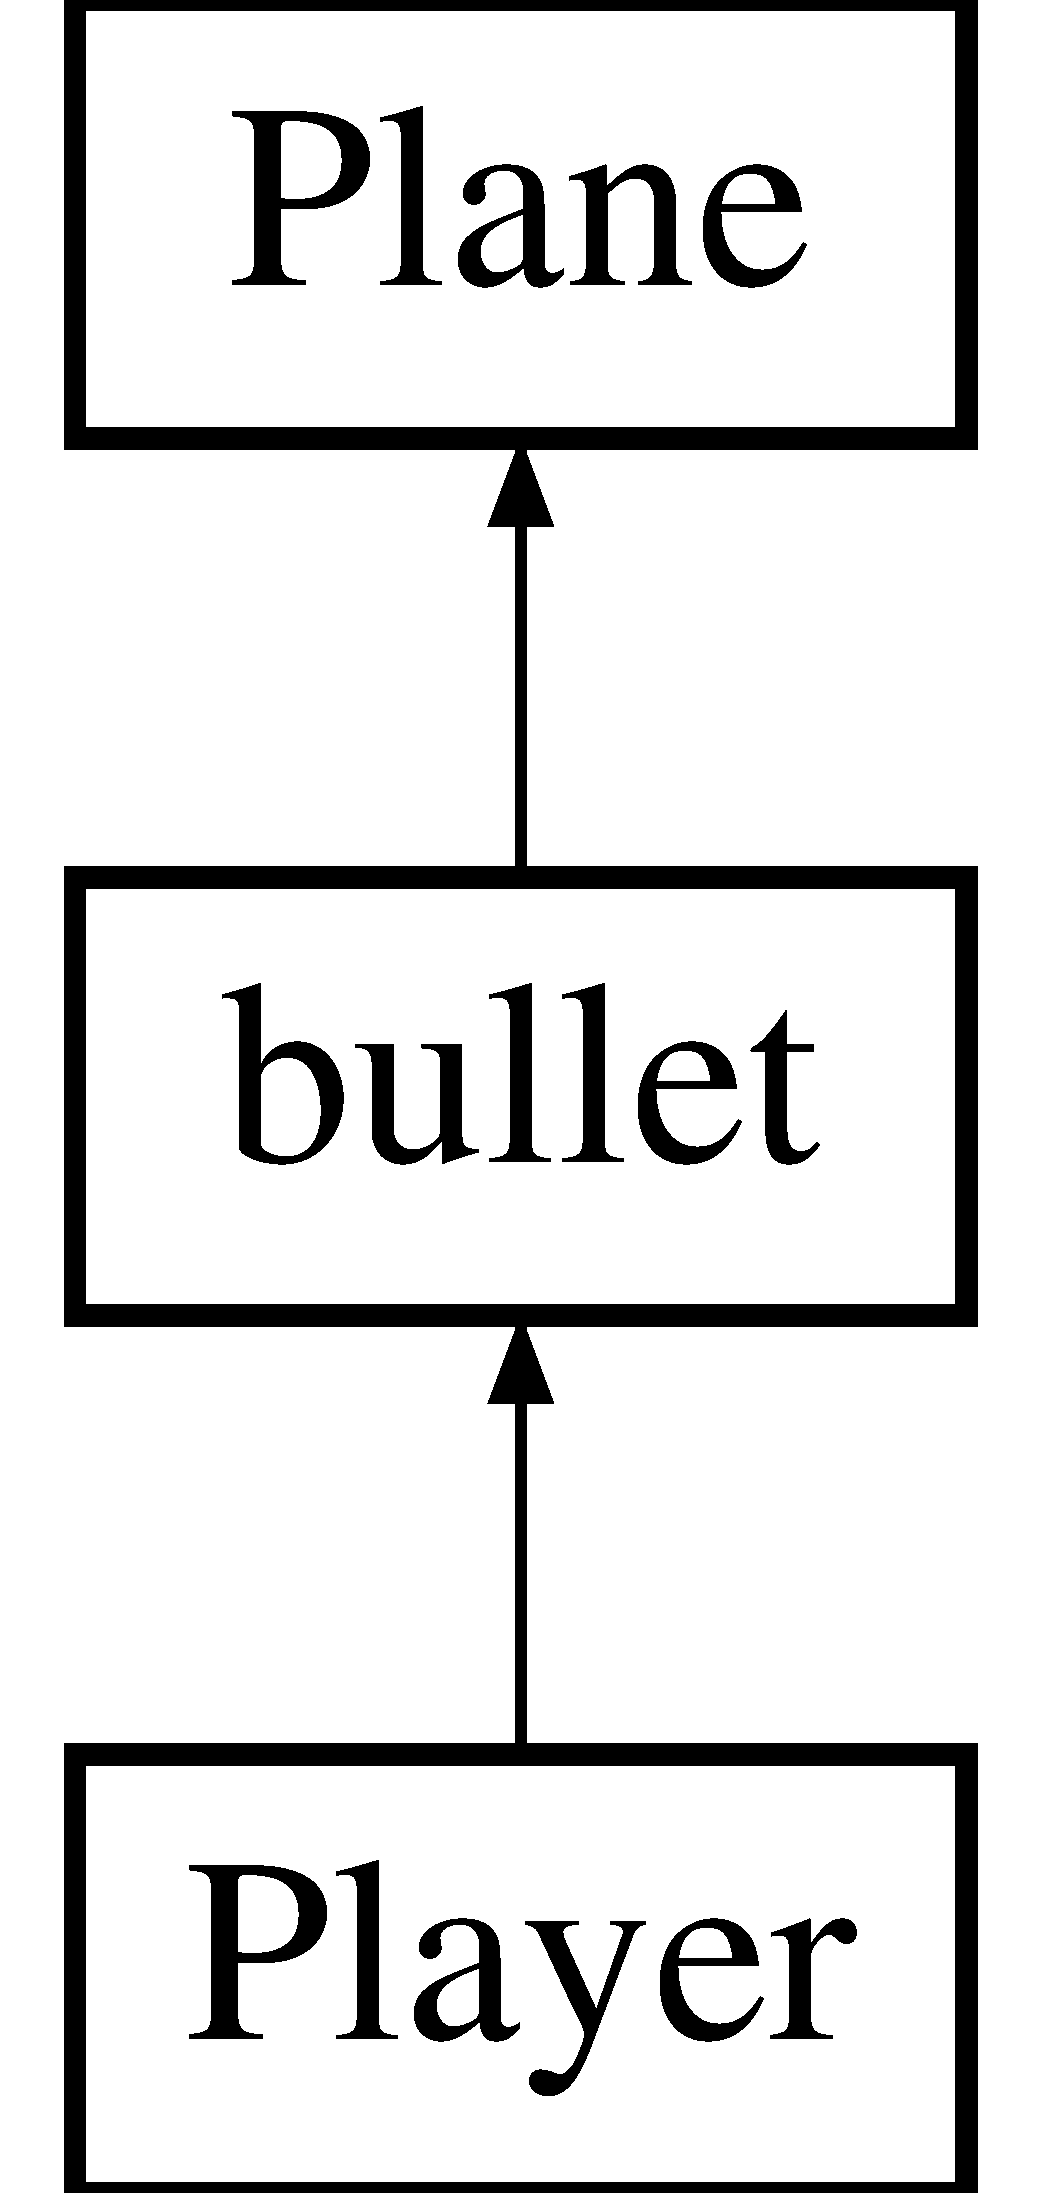
\includegraphics[height=3cm]{classPlayer}
\end{center}
\end{figure}
\subsection*{Public Member Functions}
\begin{DoxyCompactItemize}
\item 
\hyperlink{classPlayer_affe0cc3cb714f6deb4e62f0c0d3f1fd8}{Player} ()
\begin{DoxyCompactList}\small\item\em Constructor. \item\end{DoxyCompactList}\item 
\hyperlink{classPlayer_a749d2c00e1fe0f5c2746f7505a58c062}{$\sim$Player} ()
\begin{DoxyCompactList}\small\item\em Destructor. \item\end{DoxyCompactList}\item 
void \hyperlink{classPlayer_addf356ccfe6223db41eb4a06d5661a60}{doLogic} (\hyperlink{classKeyboard}{Keyboard} keyboard)
\begin{DoxyCompactList}\small\item\em Defines the movement key controls for the player object so it can be moved using a keyboard. \item\end{DoxyCompactList}\item 
void \hyperlink{classPlayer_a4c994edd3d4c3b3378501353d73e30cb}{moveBullet} ()
\begin{DoxyCompactList}\small\item\em This function initializes the movement of the \hyperlink{classbullet}{bullet} through the display. \item\end{DoxyCompactList}\end{DoxyCompactItemize}
\subsection*{Private Attributes}
\begin{DoxyCompactItemize}
\item 
int \hyperlink{classPlayer_aad33b52bfe73c4c978a3135172f286a0}{health}
\item 
int \hyperlink{classPlayer_a84469d0950bc9151404b8930e6cf0ebb}{moveSpeed}
\item 
int \hyperlink{classPlayer_a33023a67c031eceeef05268f01eae43d}{bMoveSpeed}
\end{DoxyCompactItemize}


\subsection{Constructor \& Destructor Documentation}
\hypertarget{classPlayer_affe0cc3cb714f6deb4e62f0c0d3f1fd8}{
\index{Player@{Player}!Player@{Player}}
\index{Player@{Player}!Player@{Player}}
\subsubsection[{Player}]{\setlength{\rightskip}{0pt plus 5cm}Player::Player ()}}
\label{classPlayer_affe0cc3cb714f6deb4e62f0c0d3f1fd8}


Constructor. 
\begin{DoxyParams}{Parameters}
\item[{\em No}]parameters \end{DoxyParams}
\begin{DoxyReturn}{Returns}
No return value 
\end{DoxyReturn}
\hypertarget{classPlayer_a749d2c00e1fe0f5c2746f7505a58c062}{
\index{Player@{Player}!$\sim$Player@{$\sim$Player}}
\index{$\sim$Player@{$\sim$Player}!Player@{Player}}
\subsubsection[{$\sim$Player}]{\setlength{\rightskip}{0pt plus 5cm}Player::$\sim$Player ()}}
\label{classPlayer_a749d2c00e1fe0f5c2746f7505a58c062}


Destructor. 
\begin{DoxyParams}{Parameters}
\item[{\em No}]parameters \end{DoxyParams}
\begin{DoxyReturn}{Returns}
No return value 
\end{DoxyReturn}


\subsection{Member Function Documentation}
\hypertarget{classPlayer_addf356ccfe6223db41eb4a06d5661a60}{
\index{Player@{Player}!doLogic@{doLogic}}
\index{doLogic@{doLogic}!Player@{Player}}
\subsubsection[{doLogic}]{\setlength{\rightskip}{0pt plus 5cm}Void Player::doLogic ({\bf Keyboard} {\em keyboard})}}
\label{classPlayer_addf356ccfe6223db41eb4a06d5661a60}


Defines the movement key controls for the player object so it can be moved using a keyboard. 
\begin{DoxyParams}{Parameters}
\item[{\em This}]function takes in a \hyperlink{classKeyboard}{Keyboard} object \end{DoxyParams}
\begin{DoxyReturn}{Returns}
No return value 
\end{DoxyReturn}
\hypertarget{classPlayer_a4c994edd3d4c3b3378501353d73e30cb}{
\index{Player@{Player}!moveBullet@{moveBullet}}
\index{moveBullet@{moveBullet}!Player@{Player}}
\subsubsection[{moveBullet}]{\setlength{\rightskip}{0pt plus 5cm}void Player::moveBullet ()}}
\label{classPlayer_a4c994edd3d4c3b3378501353d73e30cb}


This function initializes the movement of the \hyperlink{classbullet}{bullet} through the display. 
\begin{DoxyParams}{Parameters}
\item[{\em This}]function takes no parameters \end{DoxyParams}
\begin{DoxyReturn}{Returns}
No return value 
\end{DoxyReturn}


\subsection{Member Data Documentation}
\hypertarget{classPlayer_a33023a67c031eceeef05268f01eae43d}{
\index{Player@{Player}!bMoveSpeed@{bMoveSpeed}}
\index{bMoveSpeed@{bMoveSpeed}!Player@{Player}}
\subsubsection[{bMoveSpeed}]{\setlength{\rightskip}{0pt plus 5cm}int {\bf Player::bMoveSpeed}\hspace{0.3cm}{\ttfamily  \mbox{[}private\mbox{]}}}}
\label{classPlayer_a33023a67c031eceeef05268f01eae43d}
speed of the \hyperlink{classbullet}{bullet} \hypertarget{classPlayer_aad33b52bfe73c4c978a3135172f286a0}{
\index{Player@{Player}!health@{health}}
\index{health@{health}!Player@{Player}}
\subsubsection[{health}]{\setlength{\rightskip}{0pt plus 5cm}int {\bf Player::health}\hspace{0.3cm}{\ttfamily  \mbox{[}private\mbox{]}}}}
\label{classPlayer_aad33b52bfe73c4c978a3135172f286a0}
\hypertarget{classPlayer_a84469d0950bc9151404b8930e6cf0ebb}{
\index{Player@{Player}!moveSpeed@{moveSpeed}}
\index{moveSpeed@{moveSpeed}!Player@{Player}}
\subsubsection[{moveSpeed}]{\setlength{\rightskip}{0pt plus 5cm}int {\bf Player::moveSpeed}\hspace{0.3cm}{\ttfamily  \mbox{[}private\mbox{]}}}}
\label{classPlayer_a84469d0950bc9151404b8930e6cf0ebb}
Rate at which the player can be moved 

The documentation for this class was generated from the following files:\begin{DoxyCompactItemize}
\item 
\hyperlink{Player_8h}{Player.h}\item 
\hyperlink{Player_8cc}{Player.cc}\end{DoxyCompactItemize}

\chapter{File Documentation}
\hypertarget{Allegro_8cc}{
\section{Allegro.cc File Reference}
\label{Allegro_8cc}\index{Allegro.cc@{Allegro.cc}}
}


Implementation of the \hyperlink{classAllegro}{Allegro} class.  
{\ttfamily \#include \char`\"{}Allegro.h\char`\"{}}\par
{\ttfamily \#include $<$stdio.h$>$}\par
\subsection*{Functions}
\begin{DoxyCompactItemize}
\item 
void \hyperlink{Allegro_8cc_a3db5561fa9137b9ac3ec2133a7aa4054}{InitBackground} (\hyperlink{structBackground}{Background} \&back, float x, float y, float velx, float vely, int width, int height, int dirX, int dirY, ALLEGRO\_\-BITMAP $\ast$image)
\begin{DoxyCompactList}\small\item\em This function initializes the various background images : acts like a constructor for the background struct. \item\end{DoxyCompactList}\item 
void \hyperlink{Allegro_8cc_a21e9926b904c50aee54f966cc62dd172}{UpdateBackground} (\hyperlink{structBackground}{Background} \&back)
\begin{DoxyCompactList}\small\item\em Initializes the speed at which the background moves. \item\end{DoxyCompactList}\item 
void \hyperlink{Allegro_8cc_a5b40a7650f8818fbff0104d84a236cff}{DrawBackground} (\hyperlink{structBackground}{Background} \&back)
\begin{DoxyCompactList}\small\item\em Draws the background and makes sure it is always cycles through. \item\end{DoxyCompactList}\end{DoxyCompactItemize}
\subsection*{Variables}
\begin{DoxyCompactItemize}
\item 
const int \hyperlink{Allegro_8cc_a9649ab8139c4c2ea5c93625b30d92a05}{WIDTH} = 640
\item 
const int \hyperlink{Allegro_8cc_af728b7647e0b8c49832983a31f9a2e9b}{HEIGHT} = 480
\item 
\hyperlink{structBackground}{Background} \hyperlink{Allegro_8cc_a517498b88bc80c8256f1344b9e545844}{BG}
\item 
\hyperlink{structBackground}{Background} \hyperlink{Allegro_8cc_a03c6c56b2413727c4d2aa30878a4c9dd}{MG}
\item 
\hyperlink{structBackground}{Background} \hyperlink{Allegro_8cc_a8ab41d06d3c524eb6a6f981aec1a2f1b}{FG}
\item 
ALLEGRO\_\-BITMAP $\ast$ \hyperlink{Allegro_8cc_a8f860b073e53aafca02767b0f12fc6a0}{bgImage} = NULL
\item 
ALLEGRO\_\-BITMAP $\ast$ \hyperlink{Allegro_8cc_a524ab98ea9b49e9028efed6857dd74b5}{mgImage} = NULL
\item 
ALLEGRO\_\-BITMAP $\ast$ \hyperlink{Allegro_8cc_a371876e1de9f1b046258f5e860751c98}{fgImage} = NULL
\item 
ALLEGRO\_\-SAMPLE $\ast$ \hyperlink{Allegro_8cc_ab22ce8a8f989211c6059e8b685fa78d0}{shot} = NULL
\item 
ALLEGRO\_\-SAMPLE $\ast$ \hyperlink{Allegro_8cc_af4226d9561efb980f7c3dd74cba6ba4d}{boom} = NULL
\item 
ALLEGRO\_\-SAMPLE $\ast$ \hyperlink{Allegro_8cc_ade5ece41d11b17eb4b972f2bf0f6910b}{song} = NULL
\item 
ALLEGRO\_\-SAMPLE\_\-INSTANCE $\ast$ \hyperlink{Allegro_8cc_ae572dbdea486bf303ed756e2a1f30e0b}{songInstance} = NULL
\end{DoxyCompactItemize}


\subsection{Detailed Description}
Implementation of the \hyperlink{classAllegro}{Allegro} class. This contains the implementation of member variables and functions of the \hyperlink{classAllegro}{Allegro} class \begin{DoxyAuthor}{Author}
Wang Kangning, Jefferson Sylva-\/Iriogbe and Yuhai Shi. 
\end{DoxyAuthor}
\begin{Desc}
\item[\hyperlink{bug__bug000001}{Bug}]No known bugs. \end{Desc}


\subsection{Function Documentation}
\hypertarget{Allegro_8cc_a5b40a7650f8818fbff0104d84a236cff}{
\index{Allegro.cc@{Allegro.cc}!DrawBackground@{DrawBackground}}
\index{DrawBackground@{DrawBackground}!Allegro.cc@{Allegro.cc}}
\subsubsection[{DrawBackground}]{\setlength{\rightskip}{0pt plus 5cm}void DrawBackground ({\bf Background} \& {\em back})}}
\label{Allegro_8cc_a5b40a7650f8818fbff0104d84a236cff}


Draws the background and makes sure it is always cycles through. 
\begin{DoxyParams}{Parameters}
\item[{\em \&back}]: \hyperlink{structBackground}{Background} object with the properties of the background struct \end{DoxyParams}
\begin{DoxyReturn}{Returns}
No return value 
\end{DoxyReturn}
\hypertarget{Allegro_8cc_a3db5561fa9137b9ac3ec2133a7aa4054}{
\index{Allegro.cc@{Allegro.cc}!InitBackground@{InitBackground}}
\index{InitBackground@{InitBackground}!Allegro.cc@{Allegro.cc}}
\subsubsection[{InitBackground}]{\setlength{\rightskip}{0pt plus 5cm}void InitBackground ({\bf Background} \& {\em back}, \/  float {\em x}, \/  float {\em y}, \/  float {\em velx}, \/  float {\em vely}, \/  int {\em width}, \/  int {\em height}, \/  int {\em dirX}, \/  int {\em dirY}, \/  ALLEGRO\_\-BITMAP $\ast$ {\em image})}}
\label{Allegro_8cc_a3db5561fa9137b9ac3ec2133a7aa4054}


This function initializes the various background images : acts like a constructor for the background struct. 
\begin{DoxyParams}{Parameters}
\item[{\em \&back}]: a background object with the properties of the background struct \item[{\em x}]: x coordinate \item[{\em y}]: y coordinate \item[{\em velx}]: velocity of the background moving in the x direction \item[{\em vely}]: velocity of the background moving in the y direction \item[{\em width}]: width of the background \item[{\em height}]: height of the background \item[{\em dirX}]: direction of x \item[{\em dirY}]: direction of y \item[{\em ALLEGRO\_\-BITMAP}]: the background image \end{DoxyParams}
\begin{DoxyReturn}{Returns}
No return value 
\end{DoxyReturn}
\hypertarget{Allegro_8cc_a21e9926b904c50aee54f966cc62dd172}{
\index{Allegro.cc@{Allegro.cc}!UpdateBackground@{UpdateBackground}}
\index{UpdateBackground@{UpdateBackground}!Allegro.cc@{Allegro.cc}}
\subsubsection[{UpdateBackground}]{\setlength{\rightskip}{0pt plus 5cm}void UpdateBackground ({\bf Background} \& {\em back})}}
\label{Allegro_8cc_a21e9926b904c50aee54f966cc62dd172}


Initializes the speed at which the background moves. 
\begin{DoxyParams}{Parameters}
\item[{\em \&back}]: \hyperlink{structBackground}{Background} object with the properties of the background struct \end{DoxyParams}
\begin{DoxyReturn}{Returns}
No return value 
\end{DoxyReturn}


\subsection{Variable Documentation}
\hypertarget{Allegro_8cc_a517498b88bc80c8256f1344b9e545844}{
\index{Allegro.cc@{Allegro.cc}!BG@{BG}}
\index{BG@{BG}!Allegro.cc@{Allegro.cc}}
\subsubsection[{BG}]{\setlength{\rightskip}{0pt plus 5cm}{\bf Background} {\bf BG}}}
\label{Allegro_8cc_a517498b88bc80c8256f1344b9e545844}
\hypertarget{Allegro_8cc_a8f860b073e53aafca02767b0f12fc6a0}{
\index{Allegro.cc@{Allegro.cc}!bgImage@{bgImage}}
\index{bgImage@{bgImage}!Allegro.cc@{Allegro.cc}}
\subsubsection[{bgImage}]{\setlength{\rightskip}{0pt plus 5cm}ALLEGRO\_\-BITMAP$\ast$ {\bf bgImage} = NULL}}
\label{Allegro_8cc_a8f860b073e53aafca02767b0f12fc6a0}
\hypertarget{Allegro_8cc_af4226d9561efb980f7c3dd74cba6ba4d}{
\index{Allegro.cc@{Allegro.cc}!boom@{boom}}
\index{boom@{boom}!Allegro.cc@{Allegro.cc}}
\subsubsection[{boom}]{\setlength{\rightskip}{0pt plus 5cm}ALLEGRO\_\-SAMPLE$\ast$ {\bf boom} = NULL}}
\label{Allegro_8cc_af4226d9561efb980f7c3dd74cba6ba4d}
\hypertarget{Allegro_8cc_a8ab41d06d3c524eb6a6f981aec1a2f1b}{
\index{Allegro.cc@{Allegro.cc}!FG@{FG}}
\index{FG@{FG}!Allegro.cc@{Allegro.cc}}
\subsubsection[{FG}]{\setlength{\rightskip}{0pt plus 5cm}{\bf Background} {\bf FG}}}
\label{Allegro_8cc_a8ab41d06d3c524eb6a6f981aec1a2f1b}
\hypertarget{Allegro_8cc_a371876e1de9f1b046258f5e860751c98}{
\index{Allegro.cc@{Allegro.cc}!fgImage@{fgImage}}
\index{fgImage@{fgImage}!Allegro.cc@{Allegro.cc}}
\subsubsection[{fgImage}]{\setlength{\rightskip}{0pt plus 5cm}ALLEGRO\_\-BITMAP$\ast$ {\bf fgImage} = NULL}}
\label{Allegro_8cc_a371876e1de9f1b046258f5e860751c98}
\hypertarget{Allegro_8cc_af728b7647e0b8c49832983a31f9a2e9b}{
\index{Allegro.cc@{Allegro.cc}!HEIGHT@{HEIGHT}}
\index{HEIGHT@{HEIGHT}!Allegro.cc@{Allegro.cc}}
\subsubsection[{HEIGHT}]{\setlength{\rightskip}{0pt plus 5cm}const int {\bf HEIGHT} = 480}}
\label{Allegro_8cc_af728b7647e0b8c49832983a31f9a2e9b}
\hypertarget{Allegro_8cc_a03c6c56b2413727c4d2aa30878a4c9dd}{
\index{Allegro.cc@{Allegro.cc}!MG@{MG}}
\index{MG@{MG}!Allegro.cc@{Allegro.cc}}
\subsubsection[{MG}]{\setlength{\rightskip}{0pt plus 5cm}{\bf Background} {\bf MG}}}
\label{Allegro_8cc_a03c6c56b2413727c4d2aa30878a4c9dd}
\hypertarget{Allegro_8cc_a524ab98ea9b49e9028efed6857dd74b5}{
\index{Allegro.cc@{Allegro.cc}!mgImage@{mgImage}}
\index{mgImage@{mgImage}!Allegro.cc@{Allegro.cc}}
\subsubsection[{mgImage}]{\setlength{\rightskip}{0pt plus 5cm}ALLEGRO\_\-BITMAP$\ast$ {\bf mgImage} = NULL}}
\label{Allegro_8cc_a524ab98ea9b49e9028efed6857dd74b5}
\hypertarget{Allegro_8cc_ab22ce8a8f989211c6059e8b685fa78d0}{
\index{Allegro.cc@{Allegro.cc}!shot@{shot}}
\index{shot@{shot}!Allegro.cc@{Allegro.cc}}
\subsubsection[{shot}]{\setlength{\rightskip}{0pt plus 5cm}ALLEGRO\_\-SAMPLE$\ast$ {\bf shot} = NULL}}
\label{Allegro_8cc_ab22ce8a8f989211c6059e8b685fa78d0}
\hypertarget{Allegro_8cc_ade5ece41d11b17eb4b972f2bf0f6910b}{
\index{Allegro.cc@{Allegro.cc}!song@{song}}
\index{song@{song}!Allegro.cc@{Allegro.cc}}
\subsubsection[{song}]{\setlength{\rightskip}{0pt plus 5cm}ALLEGRO\_\-SAMPLE$\ast$ {\bf song} = NULL}}
\label{Allegro_8cc_ade5ece41d11b17eb4b972f2bf0f6910b}
\hypertarget{Allegro_8cc_ae572dbdea486bf303ed756e2a1f30e0b}{
\index{Allegro.cc@{Allegro.cc}!songInstance@{songInstance}}
\index{songInstance@{songInstance}!Allegro.cc@{Allegro.cc}}
\subsubsection[{songInstance}]{\setlength{\rightskip}{0pt plus 5cm}ALLEGRO\_\-SAMPLE\_\-INSTANCE$\ast$ {\bf songInstance} = NULL}}
\label{Allegro_8cc_ae572dbdea486bf303ed756e2a1f30e0b}
\hypertarget{Allegro_8cc_a9649ab8139c4c2ea5c93625b30d92a05}{
\index{Allegro.cc@{Allegro.cc}!WIDTH@{WIDTH}}
\index{WIDTH@{WIDTH}!Allegro.cc@{Allegro.cc}}
\subsubsection[{WIDTH}]{\setlength{\rightskip}{0pt plus 5cm}const int {\bf WIDTH} = 640}}
\label{Allegro_8cc_a9649ab8139c4c2ea5c93625b30d92a05}

\hypertarget{Allegro_8h}{
\section{Allegro.h File Reference}
\label{Allegro_8h}\index{Allegro.h@{Allegro.h}}
}


Definition of the \hyperlink{classAllegro}{Allegro} class.  
{\ttfamily \#include $<$allegro5/allegro.h$>$}\par
{\ttfamily \#include $<$allegro5/allegro\_\-image.h$>$}\par
{\ttfamily \#include $<$allegro5/allegro\_\-primitives.h$>$}\par
{\ttfamily \#include $<$allegro5/allegro\_\-font.h$>$}\par
{\ttfamily \#include $<$allegro5/allegro\_\-ttf.h$>$}\par
{\ttfamily \#include $<$allegro5/allegro\_\-audio.h$>$}\par
{\ttfamily \#include $<$allegro5/allegro\_\-acodec.h$>$}\par
{\ttfamily \#include \char`\"{}Player.h\char`\"{}}\par
{\ttfamily \#include \char`\"{}Keyboard.h\char`\"{}}\par
{\ttfamily \#include \char`\"{}Enemy.h\char`\"{}}\par
\subsection*{Classes}
\begin{DoxyCompactItemize}
\item 
class \hyperlink{classAllegro}{Allegro}
\item 
struct \hyperlink{structBackground}{Background}
\end{DoxyCompactItemize}
\subsection*{Enumerations}
\begin{DoxyCompactItemize}
\item 
enum \hyperlink{Allegro_8h_a808e5cd4979462d3bbe3070d7d147444}{States} \{ \hyperlink{Allegro_8h_a808e5cd4979462d3bbe3070d7d147444a0a041e18d712f7b239eac5375daf4a05}{TITLE}, 
\hyperlink{Allegro_8h_a808e5cd4979462d3bbe3070d7d147444a0352906d1ea1dfcd663c918f3a86755b}{PLAY}, 
\hyperlink{Allegro_8h_a808e5cd4979462d3bbe3070d7d147444a339435bd0d4a842c6107333c908a5317}{LOST}
 \}
\end{DoxyCompactItemize}


\subsection{Detailed Description}
Definition of the \hyperlink{classAllegro}{Allegro} class. This contains the public and private member variables and functions of the \hyperlink{classAllegro}{Allegro} class \begin{DoxyAuthor}{Author}
Wang Kangning, Jefferson Sylva-\/Iriogbe and Yuhai Shi. 
\end{DoxyAuthor}
\begin{Desc}
\item[\hyperlink{bug__bug000002}{Bug}]No known bugs. \end{Desc}


\subsection{Enumeration Type Documentation}
\hypertarget{Allegro_8h_a808e5cd4979462d3bbe3070d7d147444}{
\index{Allegro.h@{Allegro.h}!States@{States}}
\index{States@{States}!Allegro.h@{Allegro.h}}
\subsubsection[{States}]{\setlength{\rightskip}{0pt plus 5cm}enum {\bf States}}}
\label{Allegro_8h_a808e5cd4979462d3bbe3070d7d147444}
\begin{Desc}
\item[Enumerator: ]\par
\begin{description}
\index{TITLE@{TITLE}!Allegro.h@{Allegro.h}}\index{Allegro.h@{Allegro.h}!TITLE@{TITLE}}\item[{\em 
\hypertarget{Allegro_8h_a808e5cd4979462d3bbe3070d7d147444a0a041e18d712f7b239eac5375daf4a05}{
TITLE}
\label{Allegro_8h_a808e5cd4979462d3bbe3070d7d147444a0a041e18d712f7b239eac5375daf4a05}
}]\index{PLAY@{PLAY}!Allegro.h@{Allegro.h}}\index{Allegro.h@{Allegro.h}!PLAY@{PLAY}}\item[{\em 
\hypertarget{Allegro_8h_a808e5cd4979462d3bbe3070d7d147444a0352906d1ea1dfcd663c918f3a86755b}{
PLAY}
\label{Allegro_8h_a808e5cd4979462d3bbe3070d7d147444a0352906d1ea1dfcd663c918f3a86755b}
}]\index{LOST@{LOST}!Allegro.h@{Allegro.h}}\index{Allegro.h@{Allegro.h}!LOST@{LOST}}\item[{\em 
\hypertarget{Allegro_8h_a808e5cd4979462d3bbe3070d7d147444a339435bd0d4a842c6107333c908a5317}{
LOST}
\label{Allegro_8h_a808e5cd4979462d3bbe3070d7d147444a339435bd0d4a842c6107333c908a5317}
}]\end{description}
\end{Desc}


\hypertarget{bullet_8cc}{
\section{bullet.cc File Reference}
\label{bullet_8cc}\index{bullet.cc@{bullet.cc}}
}


Implementation of the \hyperlink{classbullet}{bullet} class.  
{\ttfamily \#include \char`\"{}bullet.h\char`\"{}}\par


\subsection{Detailed Description}
Implementation of the \hyperlink{classbullet}{bullet} class. This contains the implementation of member variables and functions of the \hyperlink{classbullet}{bullet} class \begin{DoxyAuthor}{Author}
Wang Kangning, Jefferson Sylva-\/Iriogbe and Yuhai Shi. 
\end{DoxyAuthor}
\begin{Desc}
\item[\hyperlink{bug__bug000003}{Bug}]No known bugs. \end{Desc}

\hypertarget{bullet_8h}{
\section{bullet.h File Reference}
\label{bullet_8h}\index{bullet.h@{bullet.h}}
}


Definition of the bulleyType and \hyperlink{classbullet}{bullet} class (which inherits from the \hyperlink{classPlane}{Plane} class). This contains the public and private member variables and functions of the \hyperlink{classbullet}{bullet} class.  
{\ttfamily \#include $<$string$>$}\par
{\ttfamily \#include $<$allegro5/allegro.h$>$}\par
{\ttfamily \#include $<$allegro5/allegro\_\-image.h$>$}\par
{\ttfamily \#include $<$allegro5/allegro\_\-primitives.h$>$}\par
{\ttfamily \#include \char`\"{}Plane.h\char`\"{}}\par
{\ttfamily \#include $<$list$>$}\par
\subsection*{Classes}
\begin{DoxyCompactItemize}
\item 
class \hyperlink{classbulletType}{bulletType}
\item 
class \hyperlink{classbullet}{bullet}
\end{DoxyCompactItemize}


\subsection{Detailed Description}
Definition of the bulleyType and \hyperlink{classbullet}{bullet} class (which inherits from the \hyperlink{classPlane}{Plane} class). This contains the public and private member variables and functions of the \hyperlink{classbullet}{bullet} class. \begin{DoxyAuthor}{Author}
Wang Kangning, Jefferson Sylva-\/Iriogbe and Yuhai Shi.
\end{DoxyAuthor}
\begin{Desc}
\item[\hyperlink{bug__bug000004}{Bug}]No known bugs. \end{Desc}

\hypertarget{Enemy_8cc}{
\section{Enemy.cc File Reference}
\label{Enemy_8cc}\index{Enemy.cc@{Enemy.cc}}
}


Implementation of the \hyperlink{classEnemy}{Enemy} class.  
{\ttfamily \#include \char`\"{}Enemy.h\char`\"{}}\par
{\ttfamily \#include $<$stdlib.h$>$}\par
{\ttfamily \#include $<$stdio.h$>$}\par
{\ttfamily \#include $<$time.h$>$}\par


\subsection{Detailed Description}
Implementation of the \hyperlink{classEnemy}{Enemy} class. This contains the implementation of member variables and functions of the \hyperlink{classEnemy}{Enemy} class \begin{DoxyAuthor}{Author}
Wang Kangning, Jefferson Sylva-\/Iriogbe and Yuhai Shi. 
\end{DoxyAuthor}
\begin{Desc}
\item[\hyperlink{bug__bug000005}{Bug}]No known bugs. \end{Desc}

\hypertarget{Enemy_8h}{
\section{Enemy.h File Reference}
\label{Enemy_8h}\index{Enemy.h@{Enemy.h}}
}


Definition of the \hyperlink{classEnemy}{Enemy} class.  
{\ttfamily \#include \char`\"{}EnemyOne.h\char`\"{}}\par
\subsection*{Classes}
\begin{DoxyCompactItemize}
\item 
class \hyperlink{classEnemy}{Enemy}
\end{DoxyCompactItemize}


\subsection{Detailed Description}
Definition of the \hyperlink{classEnemy}{Enemy} class. This contains the public and private member variables and functions of the \hyperlink{classEnemy}{Enemy} class \begin{DoxyAuthor}{Author}
Wang Kangning, Jefferson Sylva-\/Iriogbe and Yuhai Shi. 
\end{DoxyAuthor}
\begin{Desc}
\item[\hyperlink{bug__bug000006}{Bug}]No known bugs. \end{Desc}

\hypertarget{EnemyOne_8cc}{
\section{EnemyOne.cc File Reference}
\label{EnemyOne_8cc}\index{EnemyOne.cc@{EnemyOne.cc}}
}


Implementation of the \hyperlink{classEnemytype}{Enemytype} and \hyperlink{classEnemyOne}{EnemyOne} classes.  
{\ttfamily \#include \char`\"{}EnemyOne.h\char`\"{}}\par
{\ttfamily \#include $<$allegro5/allegro\_\-primitives.h$>$}\par


\subsection{Detailed Description}
Implementation of the \hyperlink{classEnemytype}{Enemytype} and \hyperlink{classEnemyOne}{EnemyOne} classes. This contains the implementation of member variables and functions of the \hyperlink{classEnemytype}{Enemytype} and \hyperlink{classEnemyOne}{EnemyOne} classes. \begin{DoxyAuthor}{Author}
Wang Kangning, Jefferson Sylva-\/Iriogbe and Yuhai Shi 
\end{DoxyAuthor}
\begin{Desc}
\item[\hyperlink{bug__bug000007}{Bug}]No known bugs. \end{Desc}

\hypertarget{EnemyOne_8h}{
\section{EnemyOne.h File Reference}
\label{EnemyOne_8h}\index{EnemyOne.h@{EnemyOne.h}}
}


Definition of the \hyperlink{classEnemytype}{Enemytype} and \hyperlink{classEnemyOne}{EnemyOne} classes.  
{\ttfamily \#include $<$string$>$}\par
{\ttfamily \#include $<$allegro5/allegro.h$>$}\par
{\ttfamily \#include $<$allegro5/allegro\_\-image.h$>$}\par
{\ttfamily \#include $<$stdlib.h$>$}\par
{\ttfamily \#include $<$time.h$>$}\par
{\ttfamily \#include $<$iostream$>$}\par
{\ttfamily \#include $<$list$>$}\par
\subsection*{Classes}
\begin{DoxyCompactItemize}
\item 
class \hyperlink{classEnemytype}{Enemytype}
\item 
class \hyperlink{classEnemyOne}{EnemyOne}
\end{DoxyCompactItemize}


\subsection{Detailed Description}
Definition of the \hyperlink{classEnemytype}{Enemytype} and \hyperlink{classEnemyOne}{EnemyOne} classes. This contains thepublic and private member variables and functions of the \hyperlink{classEnemytype}{Enemytype} and \hyperlink{classEnemyOne}{EnemyOne} classes \begin{DoxyAuthor}{Author}
Wang Kangning, Jefferson Sylva-\/Iriogbe and Yuhai Shi 
\end{DoxyAuthor}
\begin{Desc}
\item[\hyperlink{bug__bug000008}{Bug}]No known bugs. \end{Desc}

\hypertarget{Keyboard_8cc}{
\section{Keyboard.cc File Reference}
\label{Keyboard_8cc}\index{Keyboard.cc@{Keyboard.cc}}
}


Implementation of the \hyperlink{classKeyboard}{Keyboard} class.  
{\ttfamily \#include \char`\"{}Keyboard.h\char`\"{}}\par


\subsection{Detailed Description}
Implementation of the \hyperlink{classKeyboard}{Keyboard} class. This contains the implementation of member variables and functions of the \hyperlink{classKeyboard}{Keyboard} class \begin{DoxyAuthor}{Author}
Wang Kangning, Jefferson Sylva-\/Iriogbe and Yuhai Shi. 
\end{DoxyAuthor}
\begin{Desc}
\item[\hyperlink{bug__bug000009}{Bug}]No known bugs. \end{Desc}

\hypertarget{Keyboard_8h}{
\section{Keyboard.h File Reference}
\label{Keyboard_8h}\index{Keyboard.h@{Keyboard.h}}
}


Definition of the \hyperlink{classKeyboard}{Keyboard} Class.  
\subsection*{Classes}
\begin{DoxyCompactItemize}
\item 
class \hyperlink{classKeyboard}{Keyboard}
\end{DoxyCompactItemize}
\subsection*{Enumerations}
\begin{DoxyCompactItemize}
\item 
enum \hyperlink{Keyboard_8h_a3121b5e20cccb8e49edcbd3e9ac77712}{keys} \{ \par
\hyperlink{Keyboard_8h_a3121b5e20cccb8e49edcbd3e9ac77712aba595d8bca8bc5e67c37c0a9d89becfa}{UP}, 
\hyperlink{Keyboard_8h_a3121b5e20cccb8e49edcbd3e9ac77712adb45120aafd37a973140edee24708065}{LEFT}, 
\hyperlink{Keyboard_8h_a3121b5e20cccb8e49edcbd3e9ac77712a9b0b4a95b99523966e0e34ffdadac9da}{DOWN}, 
\hyperlink{Keyboard_8h_a3121b5e20cccb8e49edcbd3e9ac77712aec8379af7490bb9eaaf579cf17876f38}{RIGHT}, 
\par
\hyperlink{Keyboard_8h_a3121b5e20cccb8e49edcbd3e9ac77712ac08dae7edcb5c5bb959fee5971fbad95}{SPACE}, 
\hyperlink{Keyboard_8h_a3121b5e20cccb8e49edcbd3e9ac77712a951ab68bb8f7daafb78951107080904e}{ENTER}
 \}
\end{DoxyCompactItemize}


\subsection{Detailed Description}
Definition of the \hyperlink{classKeyboard}{Keyboard} Class. This contains the public and private member variables and functions of the \hyperlink{classKeyboard}{Keyboard} class \begin{DoxyAuthor}{Author}
Wang Kangning, Jefferson Sylva-\/Iriogbe and Yuhai Shi. 
\end{DoxyAuthor}
\begin{Desc}
\item[\hyperlink{bug__bug000010}{Bug}]No known bugs. \end{Desc}


\subsection{Enumeration Type Documentation}
\hypertarget{Keyboard_8h_a3121b5e20cccb8e49edcbd3e9ac77712}{
\index{Keyboard.h@{Keyboard.h}!keys@{keys}}
\index{keys@{keys}!Keyboard.h@{Keyboard.h}}
\subsubsection[{keys}]{\setlength{\rightskip}{0pt plus 5cm}enum {\bf keys}}}
\label{Keyboard_8h_a3121b5e20cccb8e49edcbd3e9ac77712}
\begin{Desc}
\item[Enumerator: ]\par
\begin{description}
\index{UP@{UP}!Keyboard.h@{Keyboard.h}}\index{Keyboard.h@{Keyboard.h}!UP@{UP}}\item[{\em 
\hypertarget{Keyboard_8h_a3121b5e20cccb8e49edcbd3e9ac77712aba595d8bca8bc5e67c37c0a9d89becfa}{
UP}
\label{Keyboard_8h_a3121b5e20cccb8e49edcbd3e9ac77712aba595d8bca8bc5e67c37c0a9d89becfa}
}]\index{LEFT@{LEFT}!Keyboard.h@{Keyboard.h}}\index{Keyboard.h@{Keyboard.h}!LEFT@{LEFT}}\item[{\em 
\hypertarget{Keyboard_8h_a3121b5e20cccb8e49edcbd3e9ac77712adb45120aafd37a973140edee24708065}{
LEFT}
\label{Keyboard_8h_a3121b5e20cccb8e49edcbd3e9ac77712adb45120aafd37a973140edee24708065}
}]\index{DOWN@{DOWN}!Keyboard.h@{Keyboard.h}}\index{Keyboard.h@{Keyboard.h}!DOWN@{DOWN}}\item[{\em 
\hypertarget{Keyboard_8h_a3121b5e20cccb8e49edcbd3e9ac77712a9b0b4a95b99523966e0e34ffdadac9da}{
DOWN}
\label{Keyboard_8h_a3121b5e20cccb8e49edcbd3e9ac77712a9b0b4a95b99523966e0e34ffdadac9da}
}]\index{RIGHT@{RIGHT}!Keyboard.h@{Keyboard.h}}\index{Keyboard.h@{Keyboard.h}!RIGHT@{RIGHT}}\item[{\em 
\hypertarget{Keyboard_8h_a3121b5e20cccb8e49edcbd3e9ac77712aec8379af7490bb9eaaf579cf17876f38}{
RIGHT}
\label{Keyboard_8h_a3121b5e20cccb8e49edcbd3e9ac77712aec8379af7490bb9eaaf579cf17876f38}
}]\index{SPACE@{SPACE}!Keyboard.h@{Keyboard.h}}\index{Keyboard.h@{Keyboard.h}!SPACE@{SPACE}}\item[{\em 
\hypertarget{Keyboard_8h_a3121b5e20cccb8e49edcbd3e9ac77712ac08dae7edcb5c5bb959fee5971fbad95}{
SPACE}
\label{Keyboard_8h_a3121b5e20cccb8e49edcbd3e9ac77712ac08dae7edcb5c5bb959fee5971fbad95}
}]\index{ENTER@{ENTER}!Keyboard.h@{Keyboard.h}}\index{Keyboard.h@{Keyboard.h}!ENTER@{ENTER}}\item[{\em 
\hypertarget{Keyboard_8h_a3121b5e20cccb8e49edcbd3e9ac77712a951ab68bb8f7daafb78951107080904e}{
ENTER}
\label{Keyboard_8h_a3121b5e20cccb8e49edcbd3e9ac77712a951ab68bb8f7daafb78951107080904e}
}]\end{description}
\end{Desc}


\hypertarget{main_8cc}{
\section{main.cc File Reference}
\label{main_8cc}\index{main.cc@{main.cc}}
}


This is the main function that calls the functions and initiates the gameplay.  
{\ttfamily \#include \char`\"{}Allegro.h\char`\"{}}\par
\subsection*{Functions}
\begin{DoxyCompactItemize}
\item 
int \hyperlink{main_8cc_ae66f6b31b5ad750f1fe042a706a4e3d4}{main} ()
\end{DoxyCompactItemize}


\subsection{Detailed Description}
This is the main function that calls the functions and initiates the gameplay. \begin{DoxyAuthor}{Author}
Wang Kangning, Jefferson Sylva-\/Iriogbe and Yuhai Shi. 
\end{DoxyAuthor}
\begin{Desc}
\item[\hyperlink{bug__bug000011}{Bug}]No known bugs. \end{Desc}


\subsection{Function Documentation}
\hypertarget{main_8cc_ae66f6b31b5ad750f1fe042a706a4e3d4}{
\index{main.cc@{main.cc}!main@{main}}
\index{main@{main}!main.cc@{main.cc}}
\subsubsection[{main}]{\setlength{\rightskip}{0pt plus 5cm}int main ()}}
\label{main_8cc_ae66f6b31b5ad750f1fe042a706a4e3d4}

\hypertarget{Plane_8cc}{
\section{Plane.cc File Reference}
\label{Plane_8cc}\index{Plane.cc@{Plane.cc}}
}


Implementation of the \hyperlink{classPlane}{Plane} class.  
{\ttfamily \#include \char`\"{}Plane.h\char`\"{}}\par
{\ttfamily \#include $<$allegro5/allegro\_\-primitives.h$>$}\par


\subsection{Detailed Description}
Implementation of the \hyperlink{classPlane}{Plane} class. This contains the implementation of member variables and functions of the \hyperlink{classPlane}{Plane} class \begin{DoxyAuthor}{Author}
Wang Kangning, Jefferson Sylva-\/Iriogbe and Yuhai Shi. 
\end{DoxyAuthor}
\begin{Desc}
\item[\hyperlink{bug__bug000012}{Bug}]No known bugs. \end{Desc}

\hypertarget{Plane_8h}{
\section{Plane.h File Reference}
\label{Plane_8h}\index{Plane.h@{Plane.h}}
}


Definition of the \hyperlink{classPlane}{Plane} class.  
{\ttfamily \#include $<$string$>$}\par
{\ttfamily \#include $<$allegro5/allegro.h$>$}\par
{\ttfamily \#include $<$allegro5/allegro\_\-image.h$>$}\par
\subsection*{Classes}
\begin{DoxyCompactItemize}
\item 
class \hyperlink{classPlane}{Plane}
\end{DoxyCompactItemize}


\subsection{Detailed Description}
Definition of the \hyperlink{classPlane}{Plane} class. This contains the public and private member variables and functions of the \hyperlink{classPlane}{Plane} class.

\begin{DoxyAuthor}{Author}
Wang Kangning, Jefferson Sylva-\/Iriogbe and Yuhai Shi 
\end{DoxyAuthor}
\begin{Desc}
\item[\hyperlink{bug__bug000013}{Bug}]No known bugs. \end{Desc}

\hypertarget{Player_8cc}{
\section{Player.cc File Reference}
\label{Player_8cc}\index{Player.cc@{Player.cc}}
}


Implementation of the \hyperlink{classPlayer}{Player} class.  
{\ttfamily \#include \char`\"{}Player.h\char`\"{}}\par


\subsection{Detailed Description}
Implementation of the \hyperlink{classPlayer}{Player} class. This contains the implementation of member variables and functions of the \hyperlink{classPlayer}{Player} class \begin{DoxyAuthor}{Author}
Wang Kangning, Jefferson Sylva-\/Iriogbe and Yuhai Shi. 
\end{DoxyAuthor}
\begin{Desc}
\item[\hyperlink{bug__bug000014}{Bug}]No known bugs. \end{Desc}

\hypertarget{Player_8h}{
\section{Player.h File Reference}
\label{Player_8h}\index{Player.h@{Player.h}}
}


Definition of the \hyperlink{classPlayer}{Player} class which inherits from the \hyperlink{classbullet}{bullet} class.  
{\ttfamily \#include \char`\"{}Keyboard.h\char`\"{}}\par
{\ttfamily \#include \char`\"{}bullet.h\char`\"{}}\par
\subsection*{Classes}
\begin{DoxyCompactItemize}
\item 
class \hyperlink{classPlayer}{Player}
\end{DoxyCompactItemize}


\subsection{Detailed Description}
Definition of the \hyperlink{classPlayer}{Player} class which inherits from the \hyperlink{classbullet}{bullet} class. This contains the public and private member variables and functions of the \hyperlink{classPlayer}{Player} class \begin{DoxyAuthor}{Author}
Wang Kangning, Jefferson Sylva-\/Iriogbe and Yuhai Shi 
\end{DoxyAuthor}
\begin{Desc}
\item[\hyperlink{bug__bug000015}{Bug}]No known bugs. \end{Desc}

\printindex
\end{document}
